\documentclass[twoside]{book}

% Packages required by doxygen
\usepackage{calc}
\usepackage{doxygen}
\usepackage{graphicx}
\usepackage[utf8]{inputenc}
\usepackage{makeidx}
\usepackage{multicol}
\usepackage{multirow}
\usepackage{textcomp}
\usepackage[table]{xcolor}

% Font selection
\usepackage[T1]{fontenc}
\usepackage{mathptmx}
\usepackage[scaled=.90]{helvet}
\usepackage{courier}
\usepackage{amssymb}
\usepackage{sectsty}
\renewcommand{\familydefault}{\sfdefault}
\allsectionsfont{%
  \fontseries{bc}\selectfont%
  \color{darkgray}%
}
\renewcommand{\DoxyLabelFont}{%
  \fontseries{bc}\selectfont%
  \color{darkgray}%
}

% Page & text layout
\usepackage{geometry}
\geometry{%
  a4paper,%
  top=2.5cm,%
  bottom=2.5cm,%
  left=2.5cm,%
  right=2.5cm%
}
\tolerance=750
\hfuzz=15pt
\hbadness=750
\setlength{\emergencystretch}{15pt}
\setlength{\parindent}{0cm}
\setlength{\parskip}{0.2cm}
\makeatletter
\renewcommand{\paragraph}{%
  \@startsection{paragraph}{4}{0ex}{-1.0ex}{1.0ex}{%
    \normalfont\normalsize\bfseries\SS@parafont%
  }%
}
\renewcommand{\subparagraph}{%
  \@startsection{subparagraph}{5}{0ex}{-1.0ex}{1.0ex}{%
    \normalfont\normalsize\bfseries\SS@subparafont%
  }%
}
\makeatother

% Headers & footers
\usepackage{fancyhdr}
\pagestyle{fancyplain}
\fancyhead[LE]{\fancyplain{}{\bfseries\thepage}}
\fancyhead[CE]{\fancyplain{}{}}
\fancyhead[RE]{\fancyplain{}{\bfseries\leftmark}}
\fancyhead[LO]{\fancyplain{}{\bfseries\rightmark}}
\fancyhead[CO]{\fancyplain{}{}}
\fancyhead[RO]{\fancyplain{}{\bfseries\thepage}}
\fancyfoot[LE]{\fancyplain{}{}}
\fancyfoot[CE]{\fancyplain{}{}}
\fancyfoot[RE]{\fancyplain{}{\bfseries\scriptsize Generated on Fri Apr 1 2016 22\-:16\-:16 for Trans\-Clust C\-P\-P First\-Draft by Doxygen }}
\fancyfoot[LO]{\fancyplain{}{\bfseries\scriptsize Generated on Fri Apr 1 2016 22\-:16\-:16 for Trans\-Clust C\-P\-P First\-Draft by Doxygen }}
\fancyfoot[CO]{\fancyplain{}{}}
\fancyfoot[RO]{\fancyplain{}{}}
\renewcommand{\footrulewidth}{0.4pt}
\renewcommand{\chaptermark}[1]{%
  \markboth{#1}{}%
}
\renewcommand{\sectionmark}[1]{%
  \markright{\thesection\ #1}%
}

% Indices & bibliography
\usepackage{natbib}
\usepackage[titles]{tocloft}
\setcounter{tocdepth}{3}
\setcounter{secnumdepth}{5}
\makeindex

% Hyperlinks (required, but should be loaded last)
\usepackage{ifpdf}
\ifpdf
  \usepackage[pdftex,pagebackref=true]{hyperref}
\else
  \usepackage[ps2pdf,pagebackref=true]{hyperref}
\fi
\hypersetup{%
  colorlinks=true,%
  linkcolor=blue,%
  citecolor=blue,%
  unicode%
}

% Custom commands
\newcommand{\clearemptydoublepage}{%
  \newpage{\pagestyle{empty}\cleardoublepage}%
}


%===== C O N T E N T S =====

\begin{document}

% Titlepage & ToC
\hypersetup{pageanchor=false}
\pagenumbering{roman}
\begin{titlepage}
\vspace*{7cm}
\begin{center}%
{\Large Trans\-Clust C\-P\-P First\-Draft }\\
\vspace*{1cm}
{\large Generated by Doxygen 1.8.6}\\
\vspace*{0.5cm}
{\small Fri Apr 1 2016 22:16:16}\\
\end{center}
\end{titlepage}
\clearemptydoublepage
\tableofcontents
\clearemptydoublepage
\pagenumbering{arabic}
\hypersetup{pageanchor=true}

%--- Begin generated contents ---
\chapter{Namespace Index}
\section{Namespace List}
Here is a list of all namespaces with brief descriptions\-:\begin{DoxyCompactList}
\item\contentsline{section}{\hyperlink{namespacefcc}{fcc} }{\pageref{namespacefcc}}{}
\item\contentsline{section}{\hyperlink{namespaceFORCE}{F\-O\-R\-C\-E} }{\pageref{namespaceFORCE}}{}
\end{DoxyCompactList}

\chapter{Class Index}
\section{Class List}
Here are the classes, structs, unions and interfaces with brief descriptions\-:\begin{DoxyCompactList}
\item\contentsline{section}{\hyperlink{classClusteringResult}{Clustering\-Result} }{\pageref{classClusteringResult}}{}
\item\contentsline{section}{\hyperlink{classConnectedComponent}{Connected\-Component} }{\pageref{classConnectedComponent}}{}
\item\contentsline{section}{\hyperlink{classResult}{Result} }{\pageref{classResult}}{}
\item\contentsline{section}{\hyperlink{classTransClust}{Trans\-Clust} }{\pageref{classTransClust}}{}
\item\contentsline{section}{\hyperlink{classTriangularMatrix}{Triangular\-Matrix} }{\pageref{classTriangularMatrix}}{}
\end{DoxyCompactList}

\chapter{File Index}
\section{File List}
Here is a list of all files with brief descriptions\-:\begin{DoxyCompactList}
\item\contentsline{section}{include/\hyperlink{ClusteringResult_8hpp}{Clustering\-Result.\-hpp} }{\pageref{ClusteringResult_8hpp}}{}
\item\contentsline{section}{include/\hyperlink{ConnectedComponent_8hpp}{Connected\-Component.\-hpp} }{\pageref{ConnectedComponent_8hpp}}{}
\item\contentsline{section}{include/\hyperlink{FindConnectedComponents_8hpp}{Find\-Connected\-Components.\-hpp} }{\pageref{FindConnectedComponents_8hpp}}{}
\item\contentsline{section}{include/\hyperlink{FORCE_8hpp}{F\-O\-R\-C\-E.\-hpp} }{\pageref{FORCE_8hpp}}{}
\item\contentsline{section}{include/\hyperlink{Result_8hpp}{Result.\-hpp} }{\pageref{Result_8hpp}}{}
\item\contentsline{section}{include/\hyperlink{TransClust_8hpp}{Trans\-Clust.\-hpp} }{\pageref{TransClust_8hpp}}{}
\item\contentsline{section}{include/\hyperlink{TriangularMatrix_8hpp}{Triangular\-Matrix.\-hpp} }{\pageref{TriangularMatrix_8hpp}}{}
\item\contentsline{section}{src/\hyperlink{ClusteringResult_8cpp}{Clustering\-Result.\-cpp} }{\pageref{ClusteringResult_8cpp}}{}
\item\contentsline{section}{src/\hyperlink{ConnectedComponent_8cpp}{Connected\-Component.\-cpp} }{\pageref{ConnectedComponent_8cpp}}{}
\item\contentsline{section}{src/\hyperlink{FindConnectedComponents_8cpp}{Find\-Connected\-Components.\-cpp} }{\pageref{FindConnectedComponents_8cpp}}{}
\item\contentsline{section}{src/\hyperlink{FORCE_8cpp}{F\-O\-R\-C\-E.\-cpp} }{\pageref{FORCE_8cpp}}{}
\item\contentsline{section}{src/\hyperlink{program_8cpp}{program.\-cpp} }{\pageref{program_8cpp}}{}
\item\contentsline{section}{src/\hyperlink{Result_8cpp}{Result.\-cpp} }{\pageref{Result_8cpp}}{}
\item\contentsline{section}{src/\hyperlink{TransClust_8cpp}{Trans\-Clust.\-cpp} }{\pageref{TransClust_8cpp}}{}
\item\contentsline{section}{src/\hyperlink{TriangularMatrix_8cpp}{Triangular\-Matrix.\-cpp} }{\pageref{TriangularMatrix_8cpp}}{}
\end{DoxyCompactList}

\chapter{Namespace Documentation}
\hypertarget{namespacefcc}{\section{fcc Namespace Reference}
\label{namespacefcc}\index{fcc@{fcc}}
}
\subsection*{Functions}
\begin{DoxyCompactItemize}
\item 
void \hyperlink{namespacefcc_a7bb6ac8b965c5b8273285865d31af94d}{find\-Connected\-Components} (const \hyperlink{classConnectedComponent}{Connected\-Component} \&cc, std\-::queue$<$ \hyperlink{classConnectedComponent}{Connected\-Component} $>$ \&ccs, const float threshold)
\item 
std\-::vector$<$ std\-::vector\\*
$<$ unsigned $>$ $>$ \hyperlink{namespacefcc_af21d20aac08ecb1a28be9244dbb525fe}{find\-Membership\-Vector} (const \hyperlink{classConnectedComponent}{Connected\-Component} \&cc, const float threshold)
\item 
void \hyperlink{namespacefcc_aabaae257f8d62570bfc4289a9483289e}{find\-Connected\-Components} (const \hyperlink{classConnectedComponent}{Connected\-Component} \&cc, const std\-::vector$<$ std\-::vector$<$ float $>$$>$ \&pos, std\-::vector$<$ \hyperlink{classConnectedComponent}{Connected\-Component} $>$ \&ccs, const float threshold)
\item 
std\-::vector$<$ std\-::vector\\*
$<$ unsigned $>$ $>$ \hyperlink{namespacefcc_a57c1a3d97ea9e78ea37513476c1b2f60}{find\-Membership\-Vector} (const \hyperlink{classConnectedComponent}{Connected\-Component} \&cc, const std\-::vector$<$ std\-::vector$<$ float $>$$>$ \&pos, std\-::vector$<$ \hyperlink{classConnectedComponent}{Connected\-Component} $>$ \&ccs, const float threshold)
\end{DoxyCompactItemize}


\subsection{Function Documentation}
\hypertarget{namespacefcc_a7bb6ac8b965c5b8273285865d31af94d}{\index{fcc@{fcc}!find\-Connected\-Components@{find\-Connected\-Components}}
\index{find\-Connected\-Components@{find\-Connected\-Components}!fcc@{fcc}}
\subsubsection[{find\-Connected\-Components}]{\setlength{\rightskip}{0pt plus 5cm}void fcc\-::find\-Connected\-Components (
\begin{DoxyParamCaption}
\item[{const {\bf Connected\-Component} \&}]{cc, }
\item[{std\-::queue$<$ {\bf Connected\-Component} $>$ \&}]{ccs, }
\item[{const float}]{threshold}
\end{DoxyParamCaption}
)}}\label{namespacefcc_a7bb6ac8b965c5b8273285865d31af94d}


Here is the call graph for this function\-:\nopagebreak
\begin{figure}[H]
\begin{center}
\leavevmode
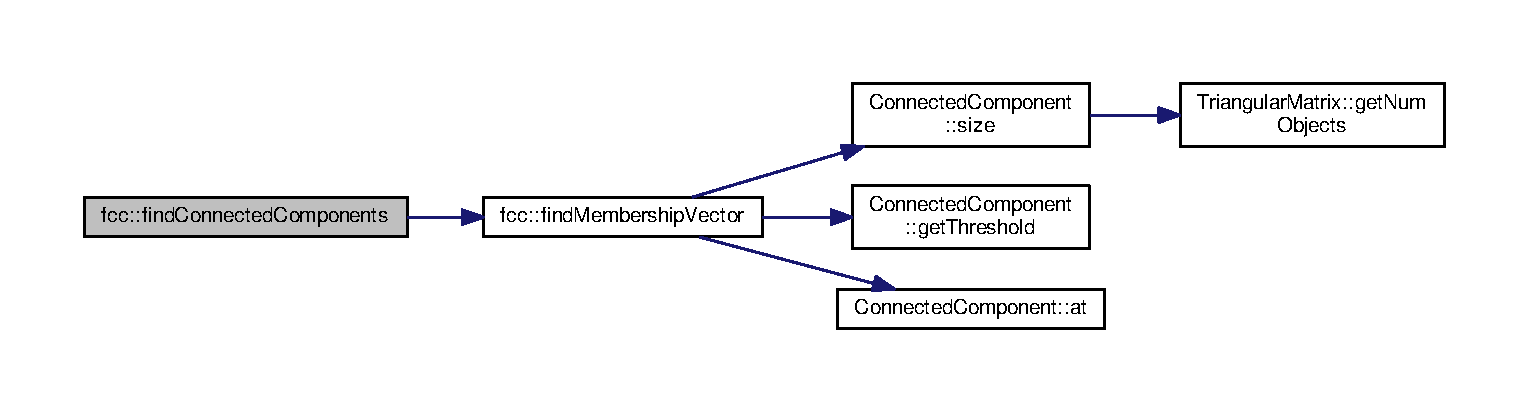
\includegraphics[width=350pt]{namespacefcc_a7bb6ac8b965c5b8273285865d31af94d_cgraph}
\end{center}
\end{figure}




Here is the caller graph for this function\-:\nopagebreak
\begin{figure}[H]
\begin{center}
\leavevmode
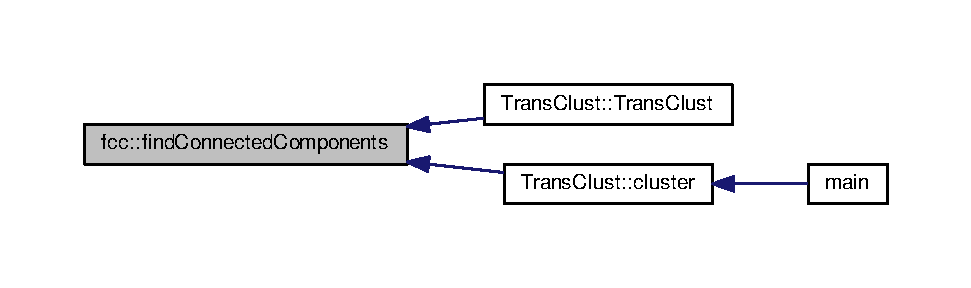
\includegraphics[width=350pt]{namespacefcc_a7bb6ac8b965c5b8273285865d31af94d_icgraph}
\end{center}
\end{figure}


\hypertarget{namespacefcc_aabaae257f8d62570bfc4289a9483289e}{\index{fcc@{fcc}!find\-Connected\-Components@{find\-Connected\-Components}}
\index{find\-Connected\-Components@{find\-Connected\-Components}!fcc@{fcc}}
\subsubsection[{find\-Connected\-Components}]{\setlength{\rightskip}{0pt plus 5cm}void fcc\-::find\-Connected\-Components (
\begin{DoxyParamCaption}
\item[{const {\bf Connected\-Component} \&}]{cc, }
\item[{const std\-::vector$<$ std\-::vector$<$ float $>$$>$ \&}]{pos, }
\item[{std\-::vector$<$ {\bf Connected\-Component} $>$ \&}]{ccs, }
\item[{const float}]{threshold}
\end{DoxyParamCaption}
)}}\label{namespacefcc_aabaae257f8d62570bfc4289a9483289e}
\hypertarget{namespacefcc_af21d20aac08ecb1a28be9244dbb525fe}{\index{fcc@{fcc}!find\-Membership\-Vector@{find\-Membership\-Vector}}
\index{find\-Membership\-Vector@{find\-Membership\-Vector}!fcc@{fcc}}
\subsubsection[{find\-Membership\-Vector}]{\setlength{\rightskip}{0pt plus 5cm}std\-::vector$<$ std\-::vector$<$ unsigned $>$ $>$ fcc\-::find\-Membership\-Vector (
\begin{DoxyParamCaption}
\item[{const {\bf Connected\-Component} \&}]{cc, }
\item[{const float}]{threshold}
\end{DoxyParamCaption}
)}}\label{namespacefcc_af21d20aac08ecb1a28be9244dbb525fe}


Here is the call graph for this function\-:\nopagebreak
\begin{figure}[H]
\begin{center}
\leavevmode
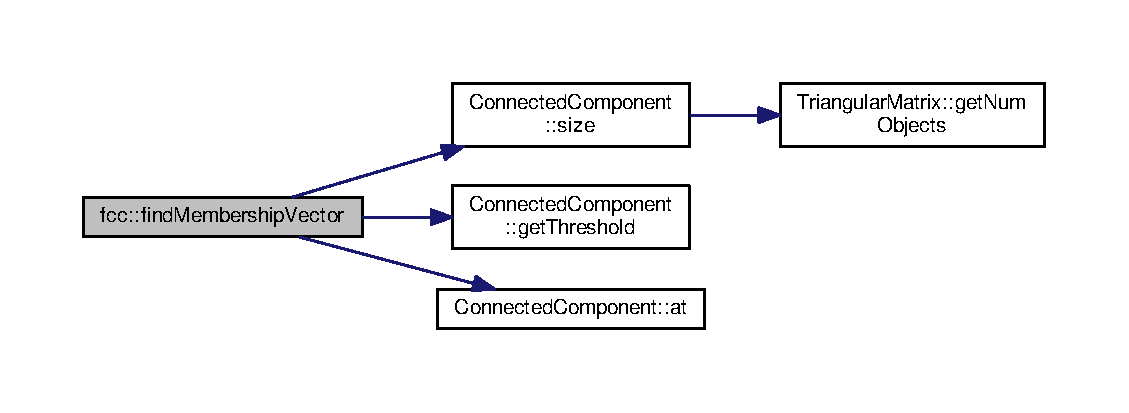
\includegraphics[width=350pt]{namespacefcc_af21d20aac08ecb1a28be9244dbb525fe_cgraph}
\end{center}
\end{figure}




Here is the caller graph for this function\-:\nopagebreak
\begin{figure}[H]
\begin{center}
\leavevmode
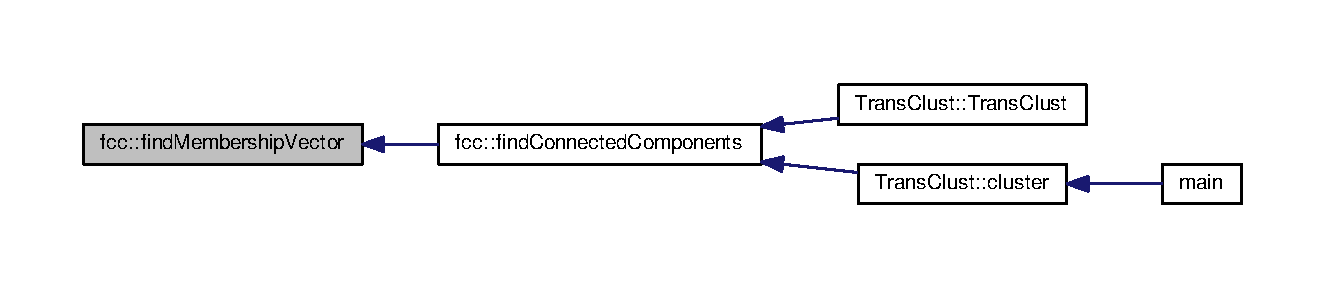
\includegraphics[width=350pt]{namespacefcc_af21d20aac08ecb1a28be9244dbb525fe_icgraph}
\end{center}
\end{figure}


\hypertarget{namespacefcc_a57c1a3d97ea9e78ea37513476c1b2f60}{\index{fcc@{fcc}!find\-Membership\-Vector@{find\-Membership\-Vector}}
\index{find\-Membership\-Vector@{find\-Membership\-Vector}!fcc@{fcc}}
\subsubsection[{find\-Membership\-Vector}]{\setlength{\rightskip}{0pt plus 5cm}std\-::vector$<$std\-::vector$<$unsigned$>$ $>$ fcc\-::find\-Membership\-Vector (
\begin{DoxyParamCaption}
\item[{const {\bf Connected\-Component} \&}]{cc, }
\item[{const std\-::vector$<$ std\-::vector$<$ float $>$$>$ \&}]{pos, }
\item[{std\-::vector$<$ {\bf Connected\-Component} $>$ \&}]{ccs, }
\item[{const float}]{threshold}
\end{DoxyParamCaption}
)}}\label{namespacefcc_a57c1a3d97ea9e78ea37513476c1b2f60}

\hypertarget{namespaceFORCE}{\section{F\-O\-R\-C\-E Namespace Reference}
\label{namespaceFORCE}\index{F\-O\-R\-C\-E@{F\-O\-R\-C\-E}}
}
\subsection*{Functions}
\begin{DoxyCompactItemize}
\item 
float \hyperlink{namespaceFORCE_aa98e605135ced38fe09c8c97a2597af0}{dist} (std\-::vector$<$ std\-::vector$<$ float $>$$>$ \&pos, unsigned i, unsigned j)
\item 
void \hyperlink{namespaceFORCE_a98853866c9b35b686d06faaeaffedff4}{layout} (const \hyperlink{classConnectedComponent}{Connected\-Component} \&cc, std\-::vector$<$ std\-::vector$<$ float $>$$>$ \&pos, float p, float f\-\_\-att, float f\-\_\-rep, unsigned R, float start\-\_\-t, unsigned dim)
\item 
\hyperlink{classClusteringResult}{Clustering\-Result} \hyperlink{namespaceFORCE_a0c6a6dbc5e4c7cc9d9c33dd884034941}{partition} (const \hyperlink{classConnectedComponent}{Connected\-Component} \&cc, std\-::vector$<$ std\-::vector$<$ float $>$$>$ \&pos, float d\-\_\-init, float d\-\_\-maximal, float s\-\_\-init, float f\-\_\-s)
\item 
std\-::vector$<$ std\-::vector\\*
$<$ unsigned $>$ $>$ \hyperlink{namespaceFORCE_ac58f3224b8bcfdce18f57ed692278f00}{geometric\-Linking} (std\-::vector$<$ std\-::vector$<$ float $>$$>$ \&pos, const float max\-Dist, const std\-::vector$<$ std\-::vector$<$ unsigned $>$$>$ \&objects)
\item 
void \hyperlink{namespaceFORCE_a4757f1fe7991d161f1deb3dafa1b933e}{D\-E\-B\-U\-G\-\_\-delta} (const \hyperlink{classConnectedComponent}{Connected\-Component} \&cc, std\-::vector$<$ std\-::vector$<$ float $>$$>$ \&pos, std\-::vector$<$ std\-::vector$<$ float $>$$>$ \&delta, unsigned r)
\item 
void \hyperlink{namespaceFORCE_a2a8c27faac3bf131cbf45212b723286e}{D\-E\-B\-U\-G\-\_\-position} (const \hyperlink{classConnectedComponent}{Connected\-Component} \&cc, std\-::vector$<$ std\-::vector$<$ float $>$$>$ \&pos, float r)
\item 
void \hyperlink{namespaceFORCE_a91fbcba5dd9ef801ef9c1b145722d7e1}{D\-E\-B\-U\-G\-\_\-linking} (std\-::vector$<$ unsigned $>$ membership, std\-::vector$<$ std\-::vector$<$ float $>$$>$ pos, float threshold, unsigned id)
\end{DoxyCompactItemize}


\subsection{Function Documentation}
\hypertarget{namespaceFORCE_a4757f1fe7991d161f1deb3dafa1b933e}{\index{F\-O\-R\-C\-E@{F\-O\-R\-C\-E}!D\-E\-B\-U\-G\-\_\-delta@{D\-E\-B\-U\-G\-\_\-delta}}
\index{D\-E\-B\-U\-G\-\_\-delta@{D\-E\-B\-U\-G\-\_\-delta}!FORCE@{F\-O\-R\-C\-E}}
\subsubsection[{D\-E\-B\-U\-G\-\_\-delta}]{\setlength{\rightskip}{0pt plus 5cm}void F\-O\-R\-C\-E\-::\-D\-E\-B\-U\-G\-\_\-delta (
\begin{DoxyParamCaption}
\item[{const {\bf Connected\-Component} \&}]{cc, }
\item[{std\-::vector$<$ std\-::vector$<$ float $>$$>$ \&}]{pos, }
\item[{std\-::vector$<$ std\-::vector$<$ float $>$$>$ \&}]{delta, }
\item[{unsigned}]{r}
\end{DoxyParamCaption}
)\hspace{0.3cm}{\ttfamily [inline]}}}\label{namespaceFORCE_a4757f1fe7991d161f1deb3dafa1b933e}


Here is the call graph for this function\-:\nopagebreak
\begin{figure}[H]
\begin{center}
\leavevmode
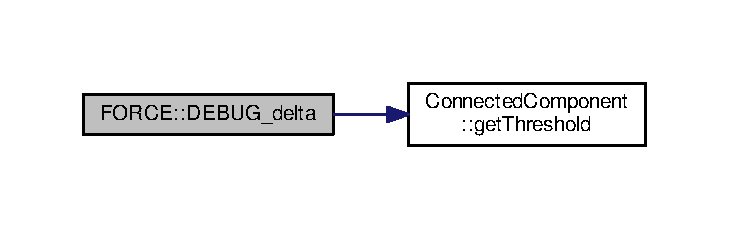
\includegraphics[width=350pt]{namespaceFORCE_a4757f1fe7991d161f1deb3dafa1b933e_cgraph}
\end{center}
\end{figure}


\hypertarget{namespaceFORCE_a91fbcba5dd9ef801ef9c1b145722d7e1}{\index{F\-O\-R\-C\-E@{F\-O\-R\-C\-E}!D\-E\-B\-U\-G\-\_\-linking@{D\-E\-B\-U\-G\-\_\-linking}}
\index{D\-E\-B\-U\-G\-\_\-linking@{D\-E\-B\-U\-G\-\_\-linking}!FORCE@{F\-O\-R\-C\-E}}
\subsubsection[{D\-E\-B\-U\-G\-\_\-linking}]{\setlength{\rightskip}{0pt plus 5cm}void F\-O\-R\-C\-E\-::\-D\-E\-B\-U\-G\-\_\-linking (
\begin{DoxyParamCaption}
\item[{std\-::vector$<$ unsigned $>$}]{membership, }
\item[{std\-::vector$<$ std\-::vector$<$ float $>$$>$}]{pos, }
\item[{float}]{threshold, }
\item[{unsigned}]{id}
\end{DoxyParamCaption}
)\hspace{0.3cm}{\ttfamily [inline]}}}\label{namespaceFORCE_a91fbcba5dd9ef801ef9c1b145722d7e1}
\hypertarget{namespaceFORCE_a2a8c27faac3bf131cbf45212b723286e}{\index{F\-O\-R\-C\-E@{F\-O\-R\-C\-E}!D\-E\-B\-U\-G\-\_\-position@{D\-E\-B\-U\-G\-\_\-position}}
\index{D\-E\-B\-U\-G\-\_\-position@{D\-E\-B\-U\-G\-\_\-position}!FORCE@{F\-O\-R\-C\-E}}
\subsubsection[{D\-E\-B\-U\-G\-\_\-position}]{\setlength{\rightskip}{0pt plus 5cm}void F\-O\-R\-C\-E\-::\-D\-E\-B\-U\-G\-\_\-position (
\begin{DoxyParamCaption}
\item[{const {\bf Connected\-Component} \&}]{cc, }
\item[{std\-::vector$<$ std\-::vector$<$ float $>$$>$ \&}]{pos, }
\item[{float}]{r}
\end{DoxyParamCaption}
)\hspace{0.3cm}{\ttfamily [inline]}}}\label{namespaceFORCE_a2a8c27faac3bf131cbf45212b723286e}


Here is the call graph for this function\-:\nopagebreak
\begin{figure}[H]
\begin{center}
\leavevmode
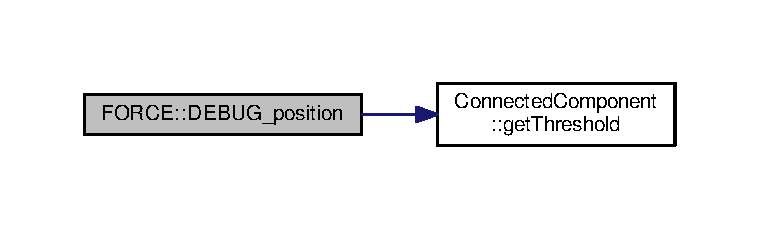
\includegraphics[width=350pt]{namespaceFORCE_a2a8c27faac3bf131cbf45212b723286e_cgraph}
\end{center}
\end{figure}


\hypertarget{namespaceFORCE_aa98e605135ced38fe09c8c97a2597af0}{\index{F\-O\-R\-C\-E@{F\-O\-R\-C\-E}!dist@{dist}}
\index{dist@{dist}!FORCE@{F\-O\-R\-C\-E}}
\subsubsection[{dist}]{\setlength{\rightskip}{0pt plus 5cm}float F\-O\-R\-C\-E\-::dist (
\begin{DoxyParamCaption}
\item[{std\-::vector$<$ std\-::vector$<$ float $>$$>$ \&}]{pos, }
\item[{unsigned}]{i, }
\item[{unsigned}]{j}
\end{DoxyParamCaption}
)}}\label{namespaceFORCE_aa98e605135ced38fe09c8c97a2597af0}


Here is the caller graph for this function\-:\nopagebreak
\begin{figure}[H]
\begin{center}
\leavevmode
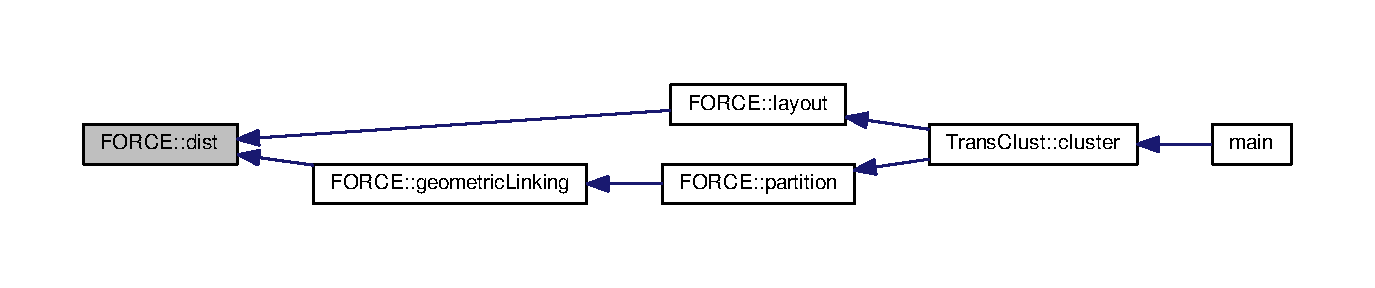
\includegraphics[width=350pt]{namespaceFORCE_aa98e605135ced38fe09c8c97a2597af0_icgraph}
\end{center}
\end{figure}


\hypertarget{namespaceFORCE_ac58f3224b8bcfdce18f57ed692278f00}{\index{F\-O\-R\-C\-E@{F\-O\-R\-C\-E}!geometric\-Linking@{geometric\-Linking}}
\index{geometric\-Linking@{geometric\-Linking}!FORCE@{F\-O\-R\-C\-E}}
\subsubsection[{geometric\-Linking}]{\setlength{\rightskip}{0pt plus 5cm}std\-::vector$<$ std\-::vector$<$ unsigned $>$ $>$ F\-O\-R\-C\-E\-::geometric\-Linking (
\begin{DoxyParamCaption}
\item[{std\-::vector$<$ std\-::vector$<$ float $>$$>$ \&}]{pos, }
\item[{const float}]{max\-Dist, }
\item[{const std\-::vector$<$ std\-::vector$<$ unsigned $>$$>$ \&}]{objects}
\end{DoxyParamCaption}
)}}\label{namespaceFORCE_ac58f3224b8bcfdce18f57ed692278f00}


Here is the call graph for this function\-:\nopagebreak
\begin{figure}[H]
\begin{center}
\leavevmode
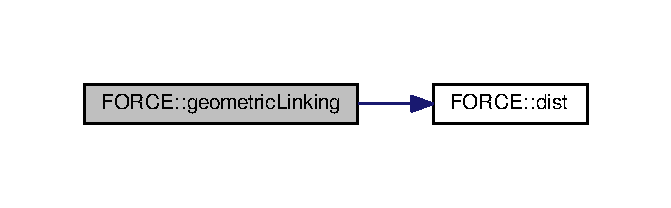
\includegraphics[width=322pt]{namespaceFORCE_ac58f3224b8bcfdce18f57ed692278f00_cgraph}
\end{center}
\end{figure}




Here is the caller graph for this function\-:\nopagebreak
\begin{figure}[H]
\begin{center}
\leavevmode
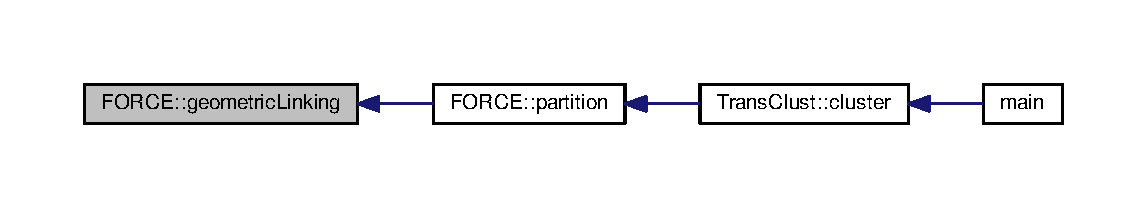
\includegraphics[width=350pt]{namespaceFORCE_ac58f3224b8bcfdce18f57ed692278f00_icgraph}
\end{center}
\end{figure}


\hypertarget{namespaceFORCE_a98853866c9b35b686d06faaeaffedff4}{\index{F\-O\-R\-C\-E@{F\-O\-R\-C\-E}!layout@{layout}}
\index{layout@{layout}!FORCE@{F\-O\-R\-C\-E}}
\subsubsection[{layout}]{\setlength{\rightskip}{0pt plus 5cm}void F\-O\-R\-C\-E\-::layout (
\begin{DoxyParamCaption}
\item[{const {\bf Connected\-Component} \&}]{cc, }
\item[{std\-::vector$<$ std\-::vector$<$ float $>$$>$ \&}]{pos, }
\item[{float}]{p, }
\item[{float}]{f\-\_\-att, }
\item[{float}]{f\-\_\-rep, }
\item[{unsigned}]{R, }
\item[{float}]{start\-\_\-t, }
\item[{unsigned}]{dim}
\end{DoxyParamCaption}
)}}\label{namespaceFORCE_a98853866c9b35b686d06faaeaffedff4}


Here is the call graph for this function\-:\nopagebreak
\begin{figure}[H]
\begin{center}
\leavevmode
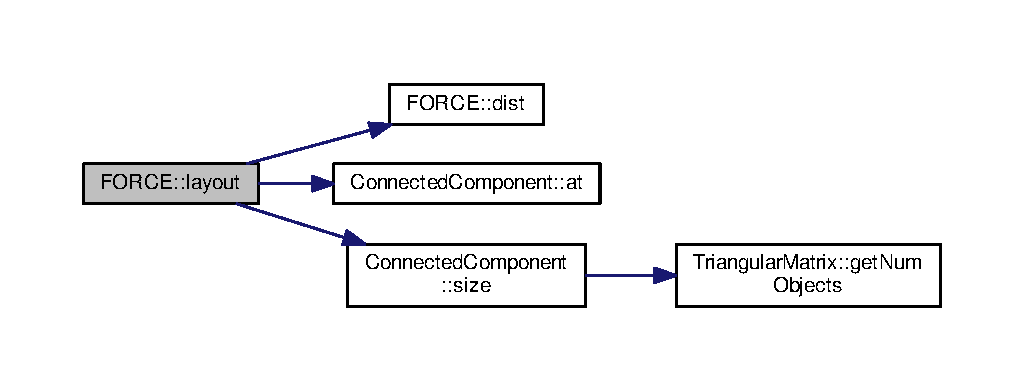
\includegraphics[width=350pt]{namespaceFORCE_a98853866c9b35b686d06faaeaffedff4_cgraph}
\end{center}
\end{figure}




Here is the caller graph for this function\-:\nopagebreak
\begin{figure}[H]
\begin{center}
\leavevmode
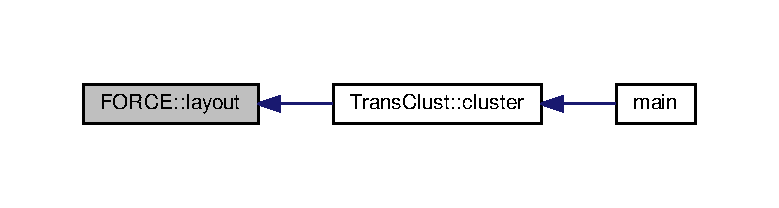
\includegraphics[width=350pt]{namespaceFORCE_a98853866c9b35b686d06faaeaffedff4_icgraph}
\end{center}
\end{figure}


\hypertarget{namespaceFORCE_a0c6a6dbc5e4c7cc9d9c33dd884034941}{\index{F\-O\-R\-C\-E@{F\-O\-R\-C\-E}!partition@{partition}}
\index{partition@{partition}!FORCE@{F\-O\-R\-C\-E}}
\subsubsection[{partition}]{\setlength{\rightskip}{0pt plus 5cm}{\bf Clustering\-Result} F\-O\-R\-C\-E\-::partition (
\begin{DoxyParamCaption}
\item[{const {\bf Connected\-Component} \&}]{cc, }
\item[{std\-::vector$<$ std\-::vector$<$ float $>$$>$ \&}]{pos, }
\item[{float}]{d\-\_\-init, }
\item[{float}]{d\-\_\-maximal, }
\item[{float}]{s\-\_\-init, }
\item[{float}]{f\-\_\-s}
\end{DoxyParamCaption}
)}}\label{namespaceFORCE_a0c6a6dbc5e4c7cc9d9c33dd884034941}


Here is the call graph for this function\-:\nopagebreak
\begin{figure}[H]
\begin{center}
\leavevmode
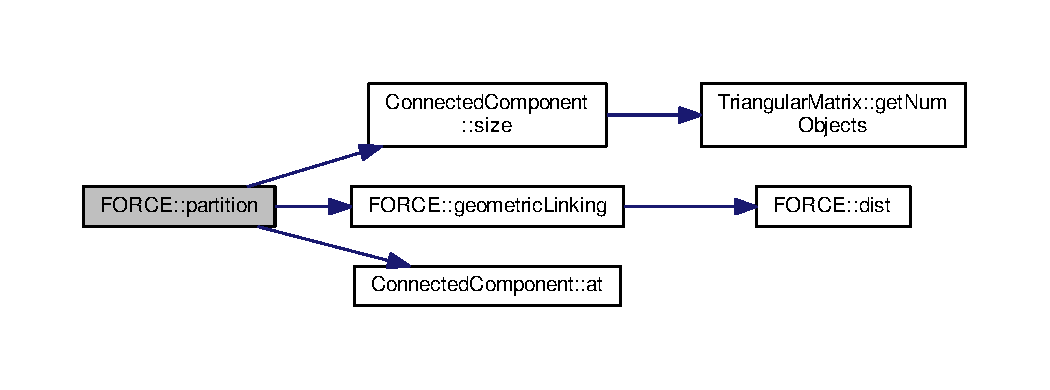
\includegraphics[width=350pt]{namespaceFORCE_a0c6a6dbc5e4c7cc9d9c33dd884034941_cgraph}
\end{center}
\end{figure}




Here is the caller graph for this function\-:\nopagebreak
\begin{figure}[H]
\begin{center}
\leavevmode
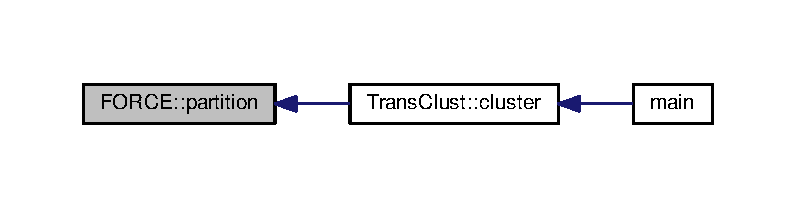
\includegraphics[width=350pt]{namespaceFORCE_a0c6a6dbc5e4c7cc9d9c33dd884034941_icgraph}
\end{center}
\end{figure}



\chapter{Class Documentation}
\hypertarget{classClusteringResult}{\section{Clustering\-Result Class Reference}
\label{classClusteringResult}\index{Clustering\-Result@{Clustering\-Result}}
}


{\ttfamily \#include $<$Clustering\-Result.\-hpp$>$}



Collaboration diagram for Clustering\-Result\-:\nopagebreak
\begin{figure}[H]
\begin{center}
\leavevmode
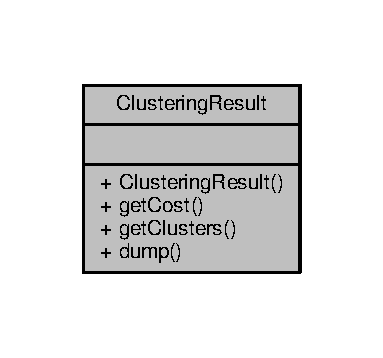
\includegraphics[width=184pt]{classClusteringResult__coll__graph}
\end{center}
\end{figure}
\subsection*{Public Member Functions}
\begin{DoxyCompactItemize}
\item 
\hyperlink{classClusteringResult_ac1d9e6b475295cea6b87dd3d85f55d37}{Clustering\-Result} (std\-::vector$<$ unsigned $>$ \&best\-\_\-cluster, float best\-\_\-cost)
\item 
float \hyperlink{classClusteringResult_aa347d753942ad533e8a1638c368769dd}{get\-Cost} ()
\item 
std\-::vector$<$ unsigned $>$ \& \hyperlink{classClusteringResult_a26acf557d1e3924438e813bd16e43f02}{get\-Clusters} ()
\item 
void \hyperlink{classClusteringResult_a9e2e35d23e98d1e89d07a4ac5223925c}{dump} ()
\end{DoxyCompactItemize}


\subsection{Constructor \& Destructor Documentation}
\hypertarget{classClusteringResult_ac1d9e6b475295cea6b87dd3d85f55d37}{\index{Clustering\-Result@{Clustering\-Result}!Clustering\-Result@{Clustering\-Result}}
\index{Clustering\-Result@{Clustering\-Result}!ClusteringResult@{Clustering\-Result}}
\subsubsection[{Clustering\-Result}]{\setlength{\rightskip}{0pt plus 5cm}Clustering\-Result\-::\-Clustering\-Result (
\begin{DoxyParamCaption}
\item[{std\-::vector$<$ unsigned $>$ \&}]{best\-\_\-cluster, }
\item[{float}]{best\-\_\-cost}
\end{DoxyParamCaption}
)}}\label{classClusteringResult_ac1d9e6b475295cea6b87dd3d85f55d37}


\subsection{Member Function Documentation}
\hypertarget{classClusteringResult_a9e2e35d23e98d1e89d07a4ac5223925c}{\index{Clustering\-Result@{Clustering\-Result}!dump@{dump}}
\index{dump@{dump}!ClusteringResult@{Clustering\-Result}}
\subsubsection[{dump}]{\setlength{\rightskip}{0pt plus 5cm}void Clustering\-Result\-::dump (
\begin{DoxyParamCaption}
{}
\end{DoxyParamCaption}
)\hspace{0.3cm}{\ttfamily [inline]}}}\label{classClusteringResult_a9e2e35d23e98d1e89d07a4ac5223925c}
\hypertarget{classClusteringResult_a26acf557d1e3924438e813bd16e43f02}{\index{Clustering\-Result@{Clustering\-Result}!get\-Clusters@{get\-Clusters}}
\index{get\-Clusters@{get\-Clusters}!ClusteringResult@{Clustering\-Result}}
\subsubsection[{get\-Clusters}]{\setlength{\rightskip}{0pt plus 5cm}std\-::vector$<$unsigned$>$\& Clustering\-Result\-::get\-Clusters (
\begin{DoxyParamCaption}
{}
\end{DoxyParamCaption}
)\hspace{0.3cm}{\ttfamily [inline]}}}\label{classClusteringResult_a26acf557d1e3924438e813bd16e43f02}


Here is the caller graph for this function\-:\nopagebreak
\begin{figure}[H]
\begin{center}
\leavevmode
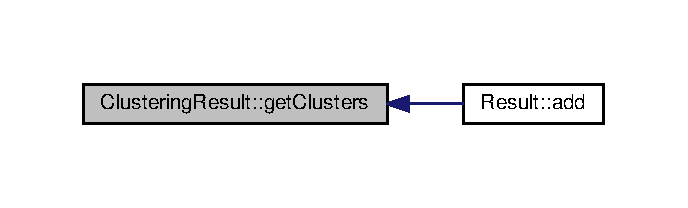
\includegraphics[width=330pt]{classClusteringResult_a26acf557d1e3924438e813bd16e43f02_icgraph}
\end{center}
\end{figure}


\hypertarget{classClusteringResult_aa347d753942ad533e8a1638c368769dd}{\index{Clustering\-Result@{Clustering\-Result}!get\-Cost@{get\-Cost}}
\index{get\-Cost@{get\-Cost}!ClusteringResult@{Clustering\-Result}}
\subsubsection[{get\-Cost}]{\setlength{\rightskip}{0pt plus 5cm}float Clustering\-Result\-::get\-Cost (
\begin{DoxyParamCaption}
{}
\end{DoxyParamCaption}
)\hspace{0.3cm}{\ttfamily [inline]}}}\label{classClusteringResult_aa347d753942ad533e8a1638c368769dd}


Here is the caller graph for this function\-:\nopagebreak
\begin{figure}[H]
\begin{center}
\leavevmode
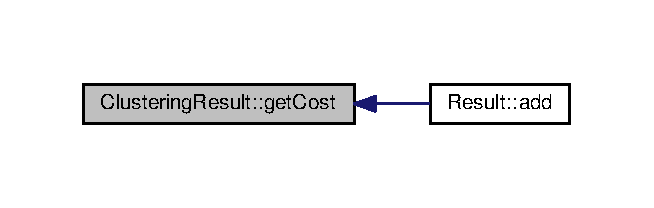
\includegraphics[width=314pt]{classClusteringResult_aa347d753942ad533e8a1638c368769dd_icgraph}
\end{center}
\end{figure}




The documentation for this class was generated from the following files\-:\begin{DoxyCompactItemize}
\item 
include/\hyperlink{ClusteringResult_8hpp}{Clustering\-Result.\-hpp}\item 
src/\hyperlink{ClusteringResult_8cpp}{Clustering\-Result.\-cpp}\end{DoxyCompactItemize}

\hypertarget{classConnectedComponent}{\section{Connected\-Component Class Reference}
\label{classConnectedComponent}\index{Connected\-Component@{Connected\-Component}}
}


{\ttfamily \#include $<$Connected\-Component.\-hpp$>$}



Collaboration diagram for Connected\-Component\-:\nopagebreak
\begin{figure}[H]
\begin{center}
\leavevmode
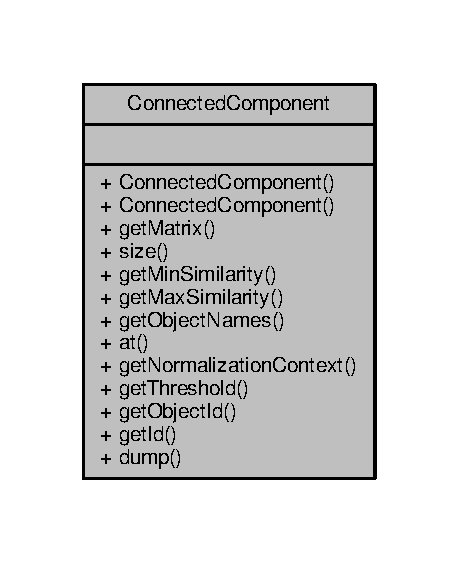
\includegraphics[width=220pt]{classConnectedComponent__coll__graph}
\end{center}
\end{figure}
\subsection*{Public Member Functions}
\begin{DoxyCompactItemize}
\item 
\hyperlink{classConnectedComponent_ab50e52197cb4972bc577580100641a63}{Connected\-Component} (const std\-::string \&filename)
\item 
\hyperlink{classConnectedComponent_ac5a046154167589817d6f6b0c0a91589}{Connected\-Component} (const \hyperlink{classConnectedComponent}{Connected\-Component} \&cc, const std\-::vector$<$ unsigned $>$ \&objects, float th)
\item 
const \hyperlink{classTriangularMatrix}{Triangular\-Matrix} \& \hyperlink{classConnectedComponent_ab44848438efe7560f1b0e923779638a3}{get\-Matrix} () const 
\item 
const unsigned \hyperlink{classConnectedComponent_a0ab1852c0c4cc9f224a59d3e8670d009}{size} () const 
\item 
const float \hyperlink{classConnectedComponent_aff31974c26d909f216620e186a978246}{get\-Min\-Similarity} () const 
\item 
const float \hyperlink{classConnectedComponent_a674bc2a6eee509ac9ea0efc45a1e4378}{get\-Max\-Similarity} () const 
\item 
const std\-::vector$<$ std\-::string $>$ \& \hyperlink{classConnectedComponent_af0f73d769badaf6331d037f7a8f3c7e6}{get\-Object\-Names} () const 
\item 
const float \hyperlink{classConnectedComponent_a079a714fe4b6ceef8c47f5fc50eaf4ea}{at} (unsigned i, unsigned j, bool normalized=true) const 
\item 
const float \hyperlink{classConnectedComponent_a9595ddaa93ca5a70fc4969357ea54b01}{get\-Normalization\-Context} () const 
\item 
const float \hyperlink{classConnectedComponent_ac2828775d06586f68945912765964698}{get\-Threshold} () const 
\item 
const unsigned \hyperlink{classConnectedComponent_a69e112172cd01a4983251e98fdc8839e}{get\-Object\-Id} (unsigned i) const 
\item 
const unsigned \hyperlink{classConnectedComponent_ab09f5a1c65d0e941934177a17f9e8df7}{get\-Id} () const 
\item 
void \hyperlink{classConnectedComponent_ac94e68d23ee387217f23c05a5ba1047c}{dump} ()
\end{DoxyCompactItemize}


\subsection{Constructor \& Destructor Documentation}
\hypertarget{classConnectedComponent_ab50e52197cb4972bc577580100641a63}{\index{Connected\-Component@{Connected\-Component}!Connected\-Component@{Connected\-Component}}
\index{Connected\-Component@{Connected\-Component}!ConnectedComponent@{Connected\-Component}}
\subsubsection[{Connected\-Component}]{\setlength{\rightskip}{0pt plus 5cm}Connected\-Component\-::\-Connected\-Component (
\begin{DoxyParamCaption}
\item[{const std\-::string \&}]{filename}
\end{DoxyParamCaption}
)}}\label{classConnectedComponent_ab50e52197cb4972bc577580100641a63}
\hypertarget{classConnectedComponent_ac5a046154167589817d6f6b0c0a91589}{\index{Connected\-Component@{Connected\-Component}!Connected\-Component@{Connected\-Component}}
\index{Connected\-Component@{Connected\-Component}!ConnectedComponent@{Connected\-Component}}
\subsubsection[{Connected\-Component}]{\setlength{\rightskip}{0pt plus 5cm}Connected\-Component\-::\-Connected\-Component (
\begin{DoxyParamCaption}
\item[{const {\bf Connected\-Component} \&}]{cc, }
\item[{const std\-::vector$<$ unsigned $>$ \&}]{objects, }
\item[{float}]{th}
\end{DoxyParamCaption}
)}}\label{classConnectedComponent_ac5a046154167589817d6f6b0c0a91589}


\subsection{Member Function Documentation}
\hypertarget{classConnectedComponent_a079a714fe4b6ceef8c47f5fc50eaf4ea}{\index{Connected\-Component@{Connected\-Component}!at@{at}}
\index{at@{at}!ConnectedComponent@{Connected\-Component}}
\subsubsection[{at}]{\setlength{\rightskip}{0pt plus 5cm}const float Connected\-Component\-::at (
\begin{DoxyParamCaption}
\item[{unsigned}]{i, }
\item[{unsigned}]{j, }
\item[{bool}]{normalized = {\ttfamily true}}
\end{DoxyParamCaption}
) const\hspace{0.3cm}{\ttfamily [inline]}}}\label{classConnectedComponent_a079a714fe4b6ceef8c47f5fc50eaf4ea}


Here is the caller graph for this function\-:\nopagebreak
\begin{figure}[H]
\begin{center}
\leavevmode
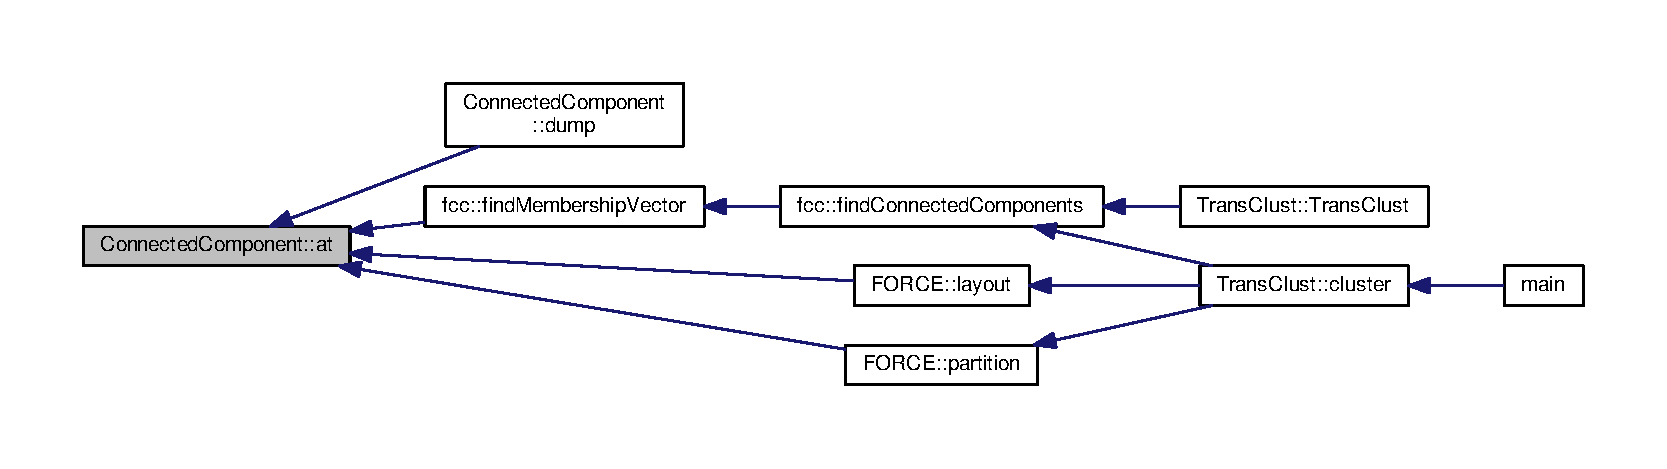
\includegraphics[width=350pt]{classConnectedComponent_a079a714fe4b6ceef8c47f5fc50eaf4ea_icgraph}
\end{center}
\end{figure}


\hypertarget{classConnectedComponent_ac94e68d23ee387217f23c05a5ba1047c}{\index{Connected\-Component@{Connected\-Component}!dump@{dump}}
\index{dump@{dump}!ConnectedComponent@{Connected\-Component}}
\subsubsection[{dump}]{\setlength{\rightskip}{0pt plus 5cm}void Connected\-Component\-::dump (
\begin{DoxyParamCaption}
{}
\end{DoxyParamCaption}
)}}\label{classConnectedComponent_ac94e68d23ee387217f23c05a5ba1047c}


Here is the call graph for this function\-:\nopagebreak
\begin{figure}[H]
\begin{center}
\leavevmode
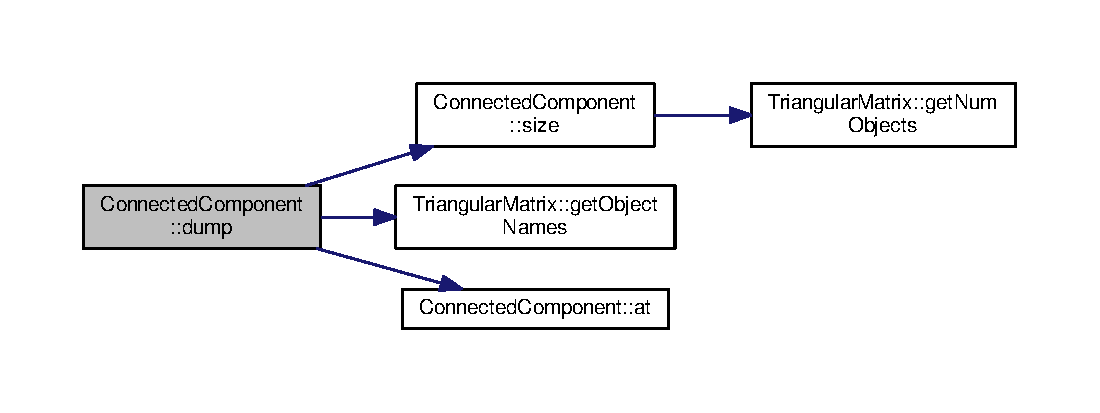
\includegraphics[width=350pt]{classConnectedComponent_ac94e68d23ee387217f23c05a5ba1047c_cgraph}
\end{center}
\end{figure}


\hypertarget{classConnectedComponent_ab09f5a1c65d0e941934177a17f9e8df7}{\index{Connected\-Component@{Connected\-Component}!get\-Id@{get\-Id}}
\index{get\-Id@{get\-Id}!ConnectedComponent@{Connected\-Component}}
\subsubsection[{get\-Id}]{\setlength{\rightskip}{0pt plus 5cm}const unsigned Connected\-Component\-::get\-Id (
\begin{DoxyParamCaption}
{}
\end{DoxyParamCaption}
) const\hspace{0.3cm}{\ttfamily [inline]}}}\label{classConnectedComponent_ab09f5a1c65d0e941934177a17f9e8df7}
\hypertarget{classConnectedComponent_ab44848438efe7560f1b0e923779638a3}{\index{Connected\-Component@{Connected\-Component}!get\-Matrix@{get\-Matrix}}
\index{get\-Matrix@{get\-Matrix}!ConnectedComponent@{Connected\-Component}}
\subsubsection[{get\-Matrix}]{\setlength{\rightskip}{0pt plus 5cm}const {\bf Triangular\-Matrix}\& Connected\-Component\-::get\-Matrix (
\begin{DoxyParamCaption}
{}
\end{DoxyParamCaption}
) const\hspace{0.3cm}{\ttfamily [inline]}}}\label{classConnectedComponent_ab44848438efe7560f1b0e923779638a3}
\hypertarget{classConnectedComponent_a674bc2a6eee509ac9ea0efc45a1e4378}{\index{Connected\-Component@{Connected\-Component}!get\-Max\-Similarity@{get\-Max\-Similarity}}
\index{get\-Max\-Similarity@{get\-Max\-Similarity}!ConnectedComponent@{Connected\-Component}}
\subsubsection[{get\-Max\-Similarity}]{\setlength{\rightskip}{0pt plus 5cm}const float Connected\-Component\-::get\-Max\-Similarity (
\begin{DoxyParamCaption}
{}
\end{DoxyParamCaption}
) const\hspace{0.3cm}{\ttfamily [inline]}}}\label{classConnectedComponent_a674bc2a6eee509ac9ea0efc45a1e4378}


Here is the call graph for this function\-:\nopagebreak
\begin{figure}[H]
\begin{center}
\leavevmode
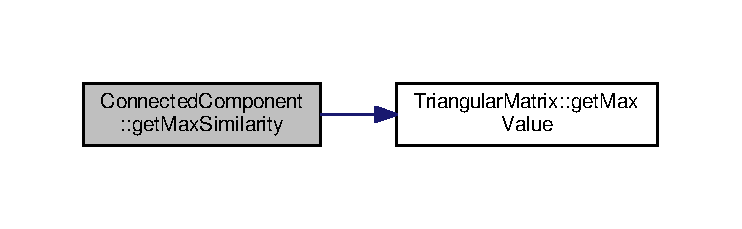
\includegraphics[width=350pt]{classConnectedComponent_a674bc2a6eee509ac9ea0efc45a1e4378_cgraph}
\end{center}
\end{figure}




Here is the caller graph for this function\-:\nopagebreak
\begin{figure}[H]
\begin{center}
\leavevmode
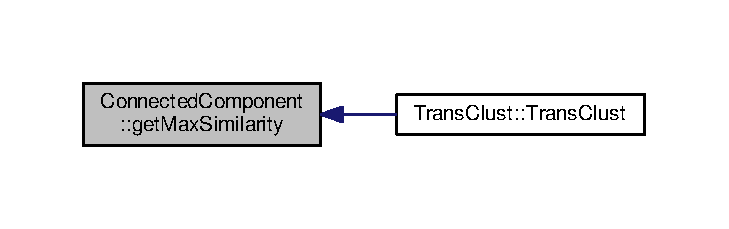
\includegraphics[width=350pt]{classConnectedComponent_a674bc2a6eee509ac9ea0efc45a1e4378_icgraph}
\end{center}
\end{figure}


\hypertarget{classConnectedComponent_aff31974c26d909f216620e186a978246}{\index{Connected\-Component@{Connected\-Component}!get\-Min\-Similarity@{get\-Min\-Similarity}}
\index{get\-Min\-Similarity@{get\-Min\-Similarity}!ConnectedComponent@{Connected\-Component}}
\subsubsection[{get\-Min\-Similarity}]{\setlength{\rightskip}{0pt plus 5cm}const float Connected\-Component\-::get\-Min\-Similarity (
\begin{DoxyParamCaption}
{}
\end{DoxyParamCaption}
) const\hspace{0.3cm}{\ttfamily [inline]}}}\label{classConnectedComponent_aff31974c26d909f216620e186a978246}


Here is the call graph for this function\-:\nopagebreak
\begin{figure}[H]
\begin{center}
\leavevmode
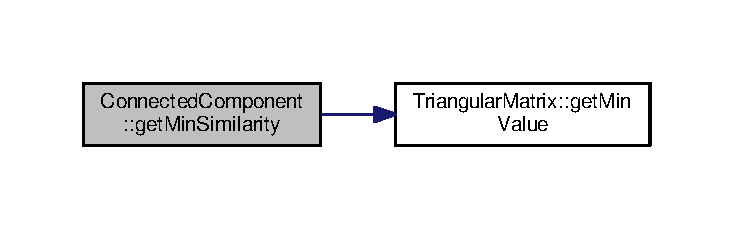
\includegraphics[width=350pt]{classConnectedComponent_aff31974c26d909f216620e186a978246_cgraph}
\end{center}
\end{figure}




Here is the caller graph for this function\-:\nopagebreak
\begin{figure}[H]
\begin{center}
\leavevmode
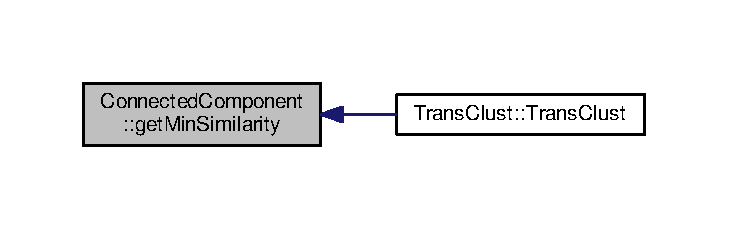
\includegraphics[width=350pt]{classConnectedComponent_aff31974c26d909f216620e186a978246_icgraph}
\end{center}
\end{figure}


\hypertarget{classConnectedComponent_a9595ddaa93ca5a70fc4969357ea54b01}{\index{Connected\-Component@{Connected\-Component}!get\-Normalization\-Context@{get\-Normalization\-Context}}
\index{get\-Normalization\-Context@{get\-Normalization\-Context}!ConnectedComponent@{Connected\-Component}}
\subsubsection[{get\-Normalization\-Context}]{\setlength{\rightskip}{0pt plus 5cm}const float Connected\-Component\-::get\-Normalization\-Context (
\begin{DoxyParamCaption}
{}
\end{DoxyParamCaption}
) const\hspace{0.3cm}{\ttfamily [inline]}}}\label{classConnectedComponent_a9595ddaa93ca5a70fc4969357ea54b01}
\hypertarget{classConnectedComponent_a69e112172cd01a4983251e98fdc8839e}{\index{Connected\-Component@{Connected\-Component}!get\-Object\-Id@{get\-Object\-Id}}
\index{get\-Object\-Id@{get\-Object\-Id}!ConnectedComponent@{Connected\-Component}}
\subsubsection[{get\-Object\-Id}]{\setlength{\rightskip}{0pt plus 5cm}const unsigned Connected\-Component\-::get\-Object\-Id (
\begin{DoxyParamCaption}
\item[{unsigned}]{i}
\end{DoxyParamCaption}
) const\hspace{0.3cm}{\ttfamily [inline]}}}\label{classConnectedComponent_a69e112172cd01a4983251e98fdc8839e}


Here is the call graph for this function\-:\nopagebreak
\begin{figure}[H]
\begin{center}
\leavevmode
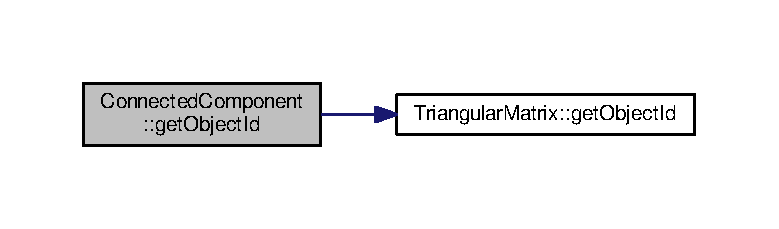
\includegraphics[width=350pt]{classConnectedComponent_a69e112172cd01a4983251e98fdc8839e_cgraph}
\end{center}
\end{figure}




Here is the caller graph for this function\-:\nopagebreak
\begin{figure}[H]
\begin{center}
\leavevmode
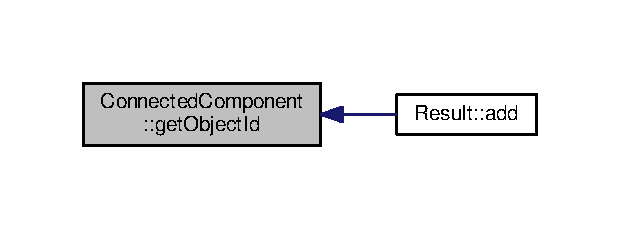
\includegraphics[width=298pt]{classConnectedComponent_a69e112172cd01a4983251e98fdc8839e_icgraph}
\end{center}
\end{figure}


\hypertarget{classConnectedComponent_af0f73d769badaf6331d037f7a8f3c7e6}{\index{Connected\-Component@{Connected\-Component}!get\-Object\-Names@{get\-Object\-Names}}
\index{get\-Object\-Names@{get\-Object\-Names}!ConnectedComponent@{Connected\-Component}}
\subsubsection[{get\-Object\-Names}]{\setlength{\rightskip}{0pt plus 5cm}const std\-::vector$<$std\-::string$>$\& Connected\-Component\-::get\-Object\-Names (
\begin{DoxyParamCaption}
{}
\end{DoxyParamCaption}
) const\hspace{0.3cm}{\ttfamily [inline]}}}\label{classConnectedComponent_af0f73d769badaf6331d037f7a8f3c7e6}


Here is the call graph for this function\-:\nopagebreak
\begin{figure}[H]
\begin{center}
\leavevmode
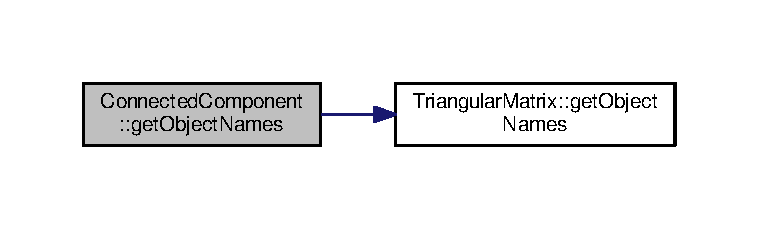
\includegraphics[width=350pt]{classConnectedComponent_af0f73d769badaf6331d037f7a8f3c7e6_cgraph}
\end{center}
\end{figure}




Here is the caller graph for this function\-:\nopagebreak
\begin{figure}[H]
\begin{center}
\leavevmode
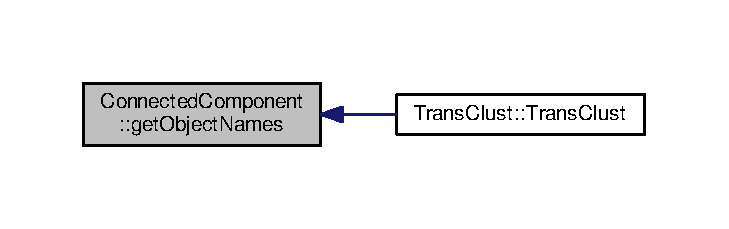
\includegraphics[width=350pt]{classConnectedComponent_af0f73d769badaf6331d037f7a8f3c7e6_icgraph}
\end{center}
\end{figure}


\hypertarget{classConnectedComponent_ac2828775d06586f68945912765964698}{\index{Connected\-Component@{Connected\-Component}!get\-Threshold@{get\-Threshold}}
\index{get\-Threshold@{get\-Threshold}!ConnectedComponent@{Connected\-Component}}
\subsubsection[{get\-Threshold}]{\setlength{\rightskip}{0pt plus 5cm}const float Connected\-Component\-::get\-Threshold (
\begin{DoxyParamCaption}
{}
\end{DoxyParamCaption}
) const\hspace{0.3cm}{\ttfamily [inline]}}}\label{classConnectedComponent_ac2828775d06586f68945912765964698}


Here is the caller graph for this function\-:\nopagebreak
\begin{figure}[H]
\begin{center}
\leavevmode
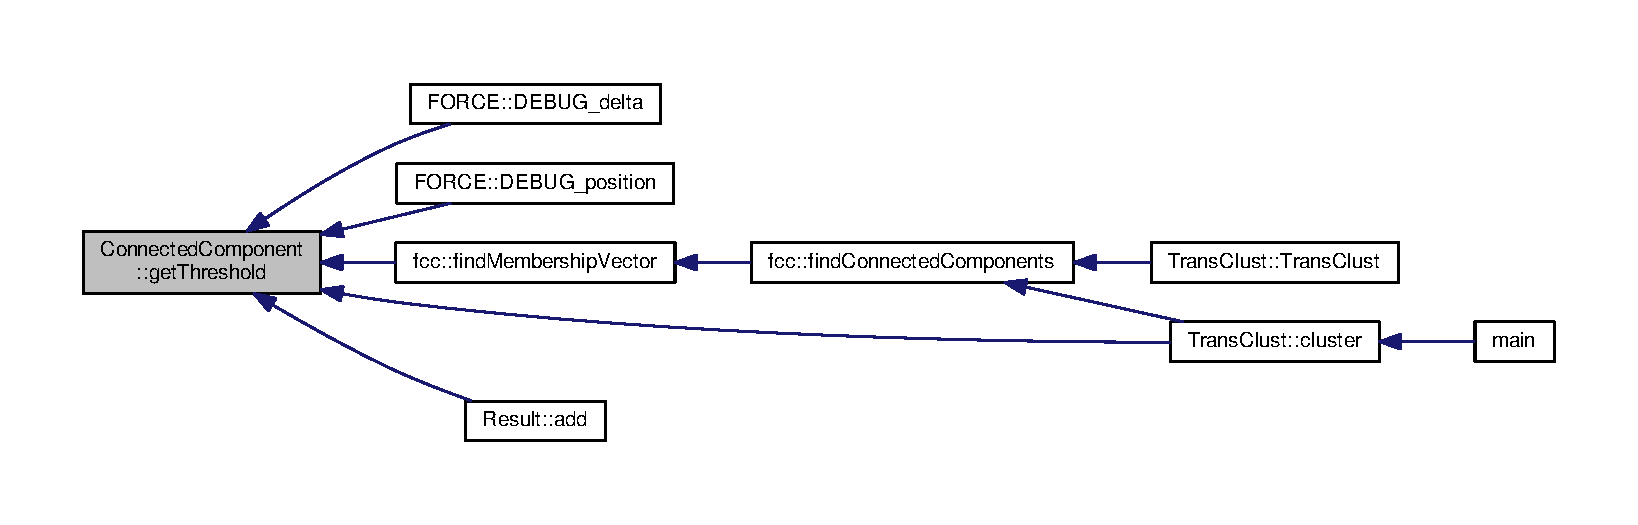
\includegraphics[width=350pt]{classConnectedComponent_ac2828775d06586f68945912765964698_icgraph}
\end{center}
\end{figure}


\hypertarget{classConnectedComponent_a0ab1852c0c4cc9f224a59d3e8670d009}{\index{Connected\-Component@{Connected\-Component}!size@{size}}
\index{size@{size}!ConnectedComponent@{Connected\-Component}}
\subsubsection[{size}]{\setlength{\rightskip}{0pt plus 5cm}const unsigned Connected\-Component\-::size (
\begin{DoxyParamCaption}
{}
\end{DoxyParamCaption}
) const\hspace{0.3cm}{\ttfamily [inline]}}}\label{classConnectedComponent_a0ab1852c0c4cc9f224a59d3e8670d009}


Here is the call graph for this function\-:\nopagebreak
\begin{figure}[H]
\begin{center}
\leavevmode
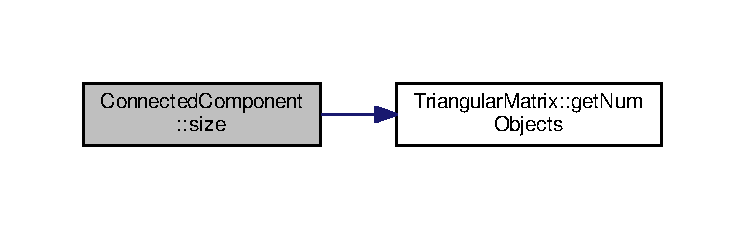
\includegraphics[width=350pt]{classConnectedComponent_a0ab1852c0c4cc9f224a59d3e8670d009_cgraph}
\end{center}
\end{figure}




Here is the caller graph for this function\-:\nopagebreak
\begin{figure}[H]
\begin{center}
\leavevmode
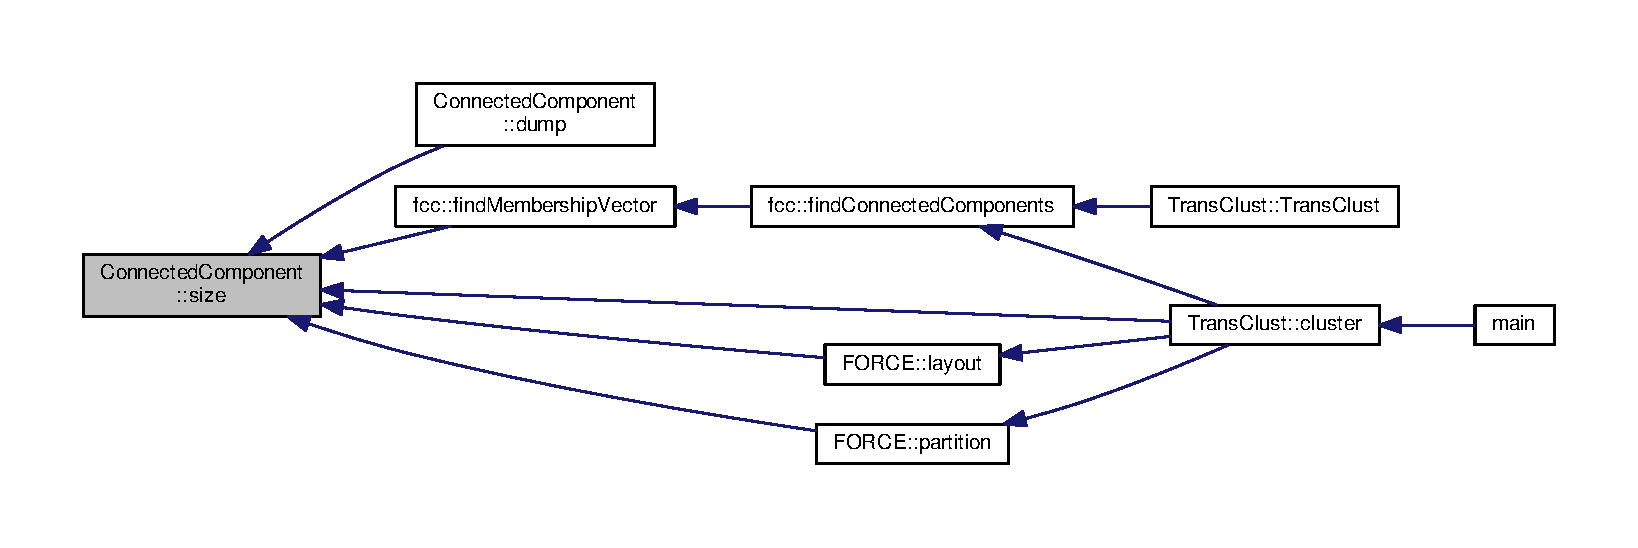
\includegraphics[width=350pt]{classConnectedComponent_a0ab1852c0c4cc9f224a59d3e8670d009_icgraph}
\end{center}
\end{figure}




The documentation for this class was generated from the following files\-:\begin{DoxyCompactItemize}
\item 
include/\hyperlink{ConnectedComponent_8hpp}{Connected\-Component.\-hpp}\item 
src/\hyperlink{ConnectedComponent_8cpp}{Connected\-Component.\-cpp}\end{DoxyCompactItemize}

\hypertarget{classResult}{\section{Result Class Reference}
\label{classResult}\index{Result@{Result}}
}


{\ttfamily \#include $<$Result.\-hpp$>$}



Collaboration diagram for Result\-:\nopagebreak
\begin{figure}[H]
\begin{center}
\leavevmode
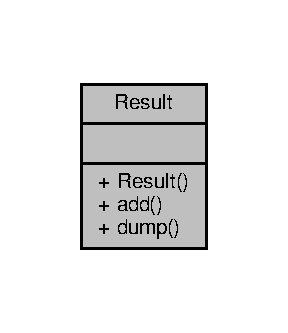
\includegraphics[width=138pt]{classResult__coll__graph}
\end{center}
\end{figure}
\subsection*{Public Member Functions}
\begin{DoxyCompactItemize}
\item 
\hyperlink{classResult_a590ded139a365b9b4994dcc0cf4813a5}{Result} (unsigned rs)
\item 
void \hyperlink{classResult_a160d1910ba8af0afff54ac0b47f249e7}{add} (\hyperlink{classConnectedComponent}{Connected\-Component} \&cc, \hyperlink{classClusteringResult}{Clustering\-Result} \&cr)
\item 
void \hyperlink{classResult_a88c390975fa3e9a4aa3b3dc87f9ba230}{dump} ()
\end{DoxyCompactItemize}


\subsection{Constructor \& Destructor Documentation}
\hypertarget{classResult_a590ded139a365b9b4994dcc0cf4813a5}{\index{Result@{Result}!Result@{Result}}
\index{Result@{Result}!Result@{Result}}
\subsubsection[{Result}]{\setlength{\rightskip}{0pt plus 5cm}Result\-::\-Result (
\begin{DoxyParamCaption}
\item[{unsigned}]{rs}
\end{DoxyParamCaption}
)}}\label{classResult_a590ded139a365b9b4994dcc0cf4813a5}


\subsection{Member Function Documentation}
\hypertarget{classResult_a160d1910ba8af0afff54ac0b47f249e7}{\index{Result@{Result}!add@{add}}
\index{add@{add}!Result@{Result}}
\subsubsection[{add}]{\setlength{\rightskip}{0pt plus 5cm}void Result\-::add (
\begin{DoxyParamCaption}
\item[{{\bf Connected\-Component} \&}]{cc, }
\item[{{\bf Clustering\-Result} \&}]{cr}
\end{DoxyParamCaption}
)}}\label{classResult_a160d1910ba8af0afff54ac0b47f249e7}


Here is the call graph for this function\-:\nopagebreak
\begin{figure}[H]
\begin{center}
\leavevmode
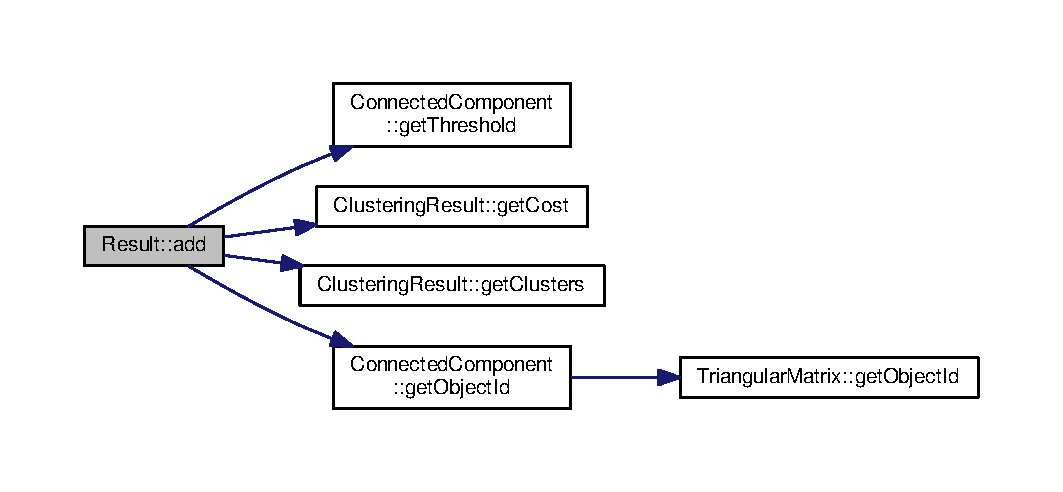
\includegraphics[width=350pt]{classResult_a160d1910ba8af0afff54ac0b47f249e7_cgraph}
\end{center}
\end{figure}


\hypertarget{classResult_a88c390975fa3e9a4aa3b3dc87f9ba230}{\index{Result@{Result}!dump@{dump}}
\index{dump@{dump}!Result@{Result}}
\subsubsection[{dump}]{\setlength{\rightskip}{0pt plus 5cm}void Result\-::dump (
\begin{DoxyParamCaption}
{}
\end{DoxyParamCaption}
)}}\label{classResult_a88c390975fa3e9a4aa3b3dc87f9ba230}


The documentation for this class was generated from the following files\-:\begin{DoxyCompactItemize}
\item 
include/\hyperlink{Result_8hpp}{Result.\-hpp}\item 
src/\hyperlink{Result_8cpp}{Result.\-cpp}\end{DoxyCompactItemize}

\hypertarget{classTransClust}{\section{Trans\-Clust Class Reference}
\label{classTransClust}\index{Trans\-Clust@{Trans\-Clust}}
}


{\ttfamily \#include $<$Trans\-Clust.\-hpp$>$}



Collaboration diagram for Trans\-Clust\-:\nopagebreak
\begin{figure}[H]
\begin{center}
\leavevmode
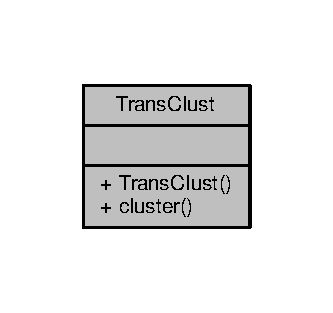
\includegraphics[width=160pt]{classTransClust__coll__graph}
\end{center}
\end{figure}
\subsection*{Public Member Functions}
\begin{DoxyCompactItemize}
\item 
\hyperlink{classTransClust_ad3b9cd0d16716606a44d0deae0c65400}{Trans\-Clust} (const std\-::string \&filename, const std\-::string ref=\char`\"{}\char`\"{}, float th\-\_\-min=0.\-0, float th\-\_\-max=0.\-0, float th\-\_\-step=0.\-0, float p=1.\-0, float f\-\_\-att=1.\-0, float f\-\_\-rep=1.\-0, unsigned R=200, unsigned dim=3, float start\-\_\-t=100, float d\-\_\-init=0.\-01, float d\-\_\-maximal=5, float s\-\_\-init=0.\-01, float f\-\_\-s=1.\-1)
\item 
void \hyperlink{classTransClust_a2a54c074c97d910e18dac65507c86cbe}{cluster} ()
\end{DoxyCompactItemize}


\subsection{Constructor \& Destructor Documentation}
\hypertarget{classTransClust_ad3b9cd0d16716606a44d0deae0c65400}{\index{Trans\-Clust@{Trans\-Clust}!Trans\-Clust@{Trans\-Clust}}
\index{Trans\-Clust@{Trans\-Clust}!TransClust@{Trans\-Clust}}
\subsubsection[{Trans\-Clust}]{\setlength{\rightskip}{0pt plus 5cm}Trans\-Clust\-::\-Trans\-Clust (
\begin{DoxyParamCaption}
\item[{const std\-::string \&}]{filename, }
\item[{const std\-::string}]{ref = {\ttfamily \char`\"{}\char`\"{}}, }
\item[{float}]{th\-\_\-min = {\ttfamily 0.0}, }
\item[{float}]{th\-\_\-max = {\ttfamily 0.0}, }
\item[{float}]{th\-\_\-step = {\ttfamily 0.0}, }
\item[{float}]{p = {\ttfamily 1.0}, }
\item[{float}]{f\-\_\-att = {\ttfamily 1.0}, }
\item[{float}]{f\-\_\-rep = {\ttfamily 1.0}, }
\item[{unsigned}]{R = {\ttfamily 200}, }
\item[{unsigned}]{dim = {\ttfamily 3}, }
\item[{float}]{start\-\_\-t = {\ttfamily 100}, }
\item[{float}]{d\-\_\-init = {\ttfamily 0.01}, }
\item[{float}]{d\-\_\-maximal = {\ttfamily 5}, }
\item[{float}]{s\-\_\-init = {\ttfamily 0.01}, }
\item[{float}]{f\-\_\-s = {\ttfamily 1.1}}
\end{DoxyParamCaption}
)}}\label{classTransClust_ad3b9cd0d16716606a44d0deae0c65400}


Here is the call graph for this function\-:\nopagebreak
\begin{figure}[H]
\begin{center}
\leavevmode
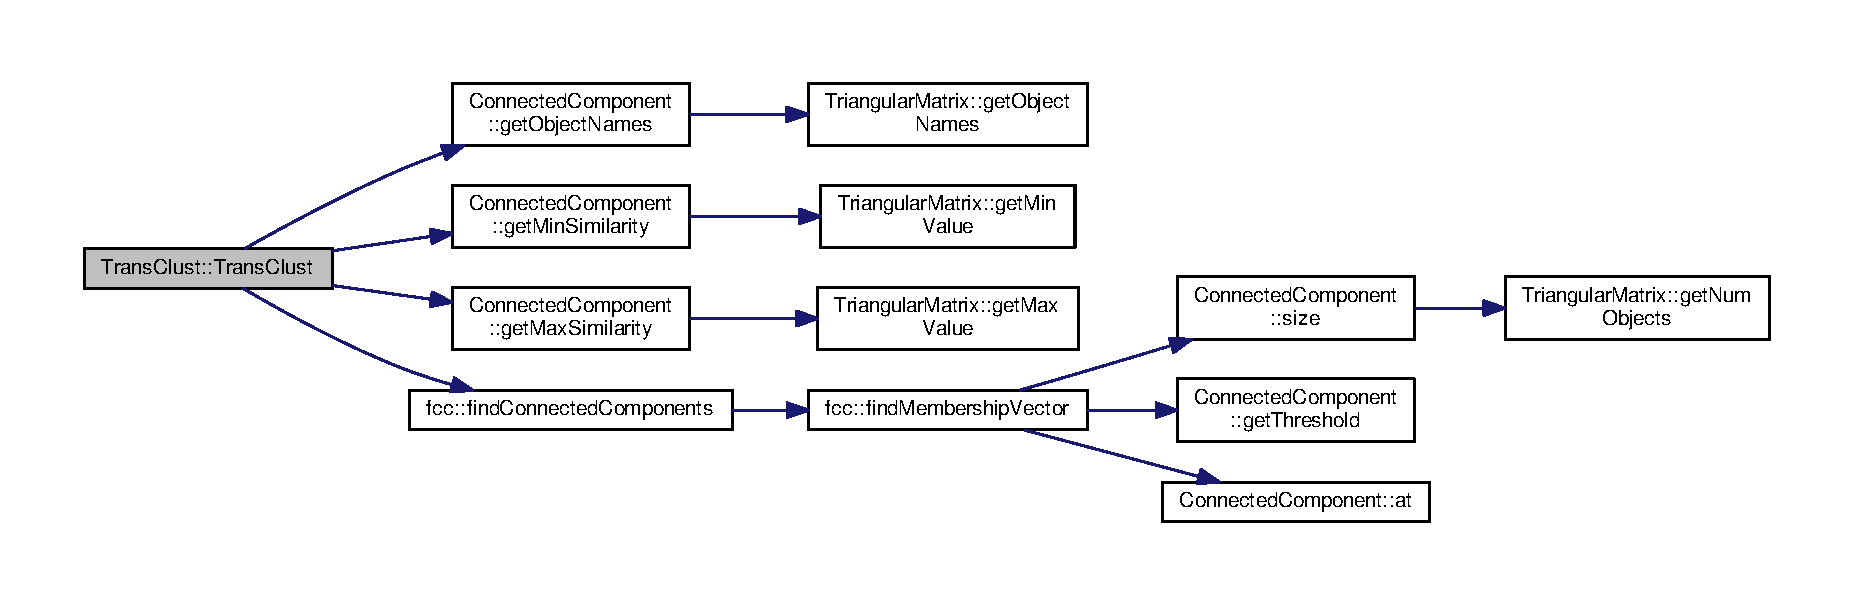
\includegraphics[width=350pt]{classTransClust_ad3b9cd0d16716606a44d0deae0c65400_cgraph}
\end{center}
\end{figure}




\subsection{Member Function Documentation}
\hypertarget{classTransClust_a2a54c074c97d910e18dac65507c86cbe}{\index{Trans\-Clust@{Trans\-Clust}!cluster@{cluster}}
\index{cluster@{cluster}!TransClust@{Trans\-Clust}}
\subsubsection[{cluster}]{\setlength{\rightskip}{0pt plus 5cm}void Trans\-Clust\-::cluster (
\begin{DoxyParamCaption}
{}
\end{DoxyParamCaption}
)}}\label{classTransClust_a2a54c074c97d910e18dac65507c86cbe}


Here is the call graph for this function\-:\nopagebreak
\begin{figure}[H]
\begin{center}
\leavevmode
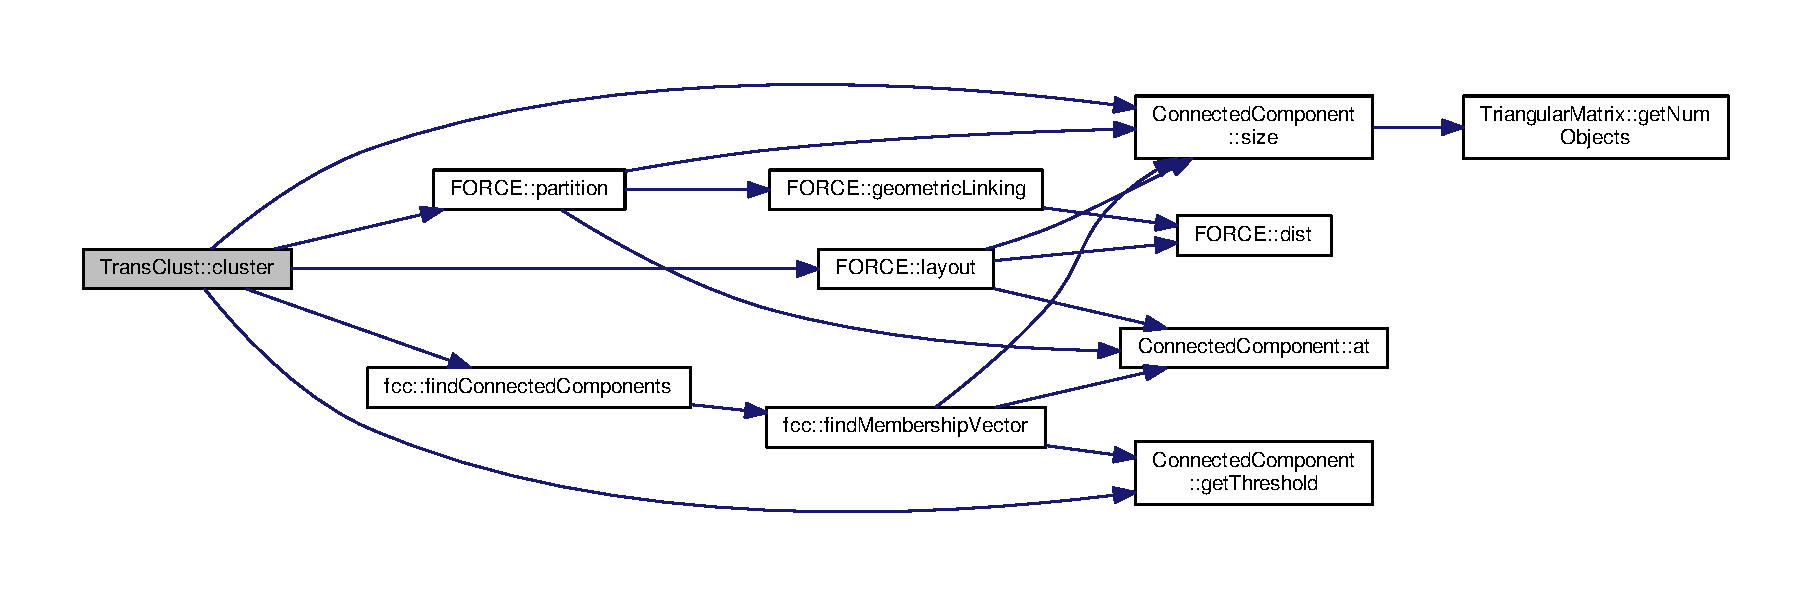
\includegraphics[width=350pt]{classTransClust_a2a54c074c97d910e18dac65507c86cbe_cgraph}
\end{center}
\end{figure}




Here is the caller graph for this function\-:\nopagebreak
\begin{figure}[H]
\begin{center}
\leavevmode
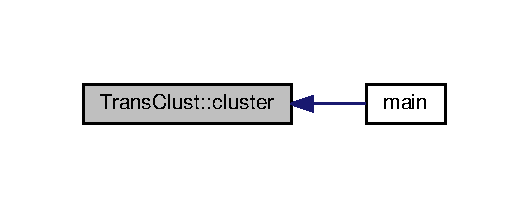
\includegraphics[width=254pt]{classTransClust_a2a54c074c97d910e18dac65507c86cbe_icgraph}
\end{center}
\end{figure}




The documentation for this class was generated from the following files\-:\begin{DoxyCompactItemize}
\item 
include/\hyperlink{TransClust_8hpp}{Trans\-Clust.\-hpp}\item 
src/\hyperlink{TransClust_8cpp}{Trans\-Clust.\-cpp}\end{DoxyCompactItemize}

\hypertarget{classTriangularMatrix}{\section{Triangular\-Matrix Class Reference}
\label{classTriangularMatrix}\index{Triangular\-Matrix@{Triangular\-Matrix}}
}


{\ttfamily \#include $<$Triangular\-Matrix.\-hpp$>$}



Collaboration diagram for Triangular\-Matrix\-:\nopagebreak
\begin{figure}[H]
\begin{center}
\leavevmode
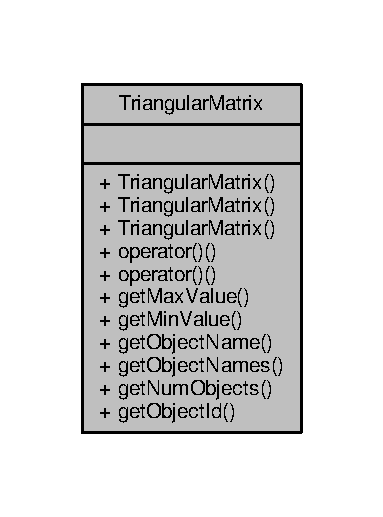
\includegraphics[width=184pt]{classTriangularMatrix__coll__graph}
\end{center}
\end{figure}
\subsection*{Public Member Functions}
\begin{DoxyCompactItemize}
\item 
\hyperlink{classTriangularMatrix_ad36af401c342c0e6dd4ba6f11516869a}{Triangular\-Matrix} (const \hyperlink{classTriangularMatrix}{Triangular\-Matrix} \&m, const std\-::vector$<$ unsigned $>$ \&objects)
\item 
\hyperlink{classTriangularMatrix_a8f4116f20aed58d3710bc42bb5ff8d87}{Triangular\-Matrix} (const std\-::string \&filename)
\item 
\hyperlink{classTriangularMatrix_a6603e4d334209fba3aecfa080bec63e7}{Triangular\-Matrix} (const std\-::vector$<$ std\-::vector$<$ float $>$$>$ \&pos)
\item 
float \& \hyperlink{classTriangularMatrix_adba103bc50d20c4fd623ee0d00d94cc4}{operator()} (unsigned i, unsigned j)
\item 
const float \& \hyperlink{classTriangularMatrix_a61d203934af7655e8406b623326cf8e1}{operator()} (unsigned i, unsigned j) const 
\item 
float \hyperlink{classTriangularMatrix_a1f93bf63a6c6c09d5130ab3111aaab05}{get\-Max\-Value} () const 
\item 
float \hyperlink{classTriangularMatrix_adfcd136b2d1e437fe86eee93e8d5dcee}{get\-Min\-Value} () const 
\item 
const std\-::string \hyperlink{classTriangularMatrix_a13b74e86bd006c503c9a2958b2b93a3a}{get\-Object\-Name} (unsigned i) const 
\item 
const std\-::vector$<$ std\-::string $>$ \& \hyperlink{classTriangularMatrix_a8786092d7b7c58613b6e19384c7ebfcb}{get\-Object\-Names} () const 
\item 
const unsigned \hyperlink{classTriangularMatrix_a5040afab8fb04018c02dc2532401fab1}{get\-Num\-Objects} () const 
\item 
const unsigned \hyperlink{classTriangularMatrix_aced0b17dd812119356bc0a0e601b3fff}{get\-Object\-Id} (unsigned i) const 
\end{DoxyCompactItemize}


\subsection{Constructor \& Destructor Documentation}
\hypertarget{classTriangularMatrix_ad36af401c342c0e6dd4ba6f11516869a}{\index{Triangular\-Matrix@{Triangular\-Matrix}!Triangular\-Matrix@{Triangular\-Matrix}}
\index{Triangular\-Matrix@{Triangular\-Matrix}!TriangularMatrix@{Triangular\-Matrix}}
\subsubsection[{Triangular\-Matrix}]{\setlength{\rightskip}{0pt plus 5cm}Triangular\-Matrix\-::\-Triangular\-Matrix (
\begin{DoxyParamCaption}
\item[{const {\bf Triangular\-Matrix} \&}]{m, }
\item[{const std\-::vector$<$ unsigned $>$ \&}]{objects}
\end{DoxyParamCaption}
)}}\label{classTriangularMatrix_ad36af401c342c0e6dd4ba6f11516869a}


Here is the call graph for this function\-:\nopagebreak
\begin{figure}[H]
\begin{center}
\leavevmode
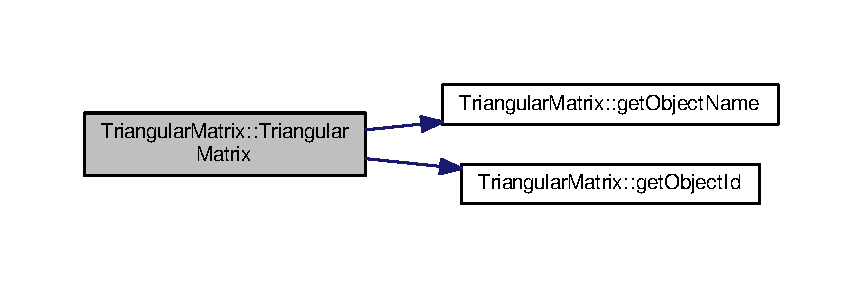
\includegraphics[width=350pt]{classTriangularMatrix_ad36af401c342c0e6dd4ba6f11516869a_cgraph}
\end{center}
\end{figure}


\hypertarget{classTriangularMatrix_a8f4116f20aed58d3710bc42bb5ff8d87}{\index{Triangular\-Matrix@{Triangular\-Matrix}!Triangular\-Matrix@{Triangular\-Matrix}}
\index{Triangular\-Matrix@{Triangular\-Matrix}!TriangularMatrix@{Triangular\-Matrix}}
\subsubsection[{Triangular\-Matrix}]{\setlength{\rightskip}{0pt plus 5cm}Triangular\-Matrix\-::\-Triangular\-Matrix (
\begin{DoxyParamCaption}
\item[{const std\-::string \&}]{filename}
\end{DoxyParamCaption}
)}}\label{classTriangularMatrix_a8f4116f20aed58d3710bc42bb5ff8d87}
\hypertarget{classTriangularMatrix_a6603e4d334209fba3aecfa080bec63e7}{\index{Triangular\-Matrix@{Triangular\-Matrix}!Triangular\-Matrix@{Triangular\-Matrix}}
\index{Triangular\-Matrix@{Triangular\-Matrix}!TriangularMatrix@{Triangular\-Matrix}}
\subsubsection[{Triangular\-Matrix}]{\setlength{\rightskip}{0pt plus 5cm}Triangular\-Matrix\-::\-Triangular\-Matrix (
\begin{DoxyParamCaption}
\item[{const std\-::vector$<$ std\-::vector$<$ float $>$$>$ \&}]{pos}
\end{DoxyParamCaption}
)}}\label{classTriangularMatrix_a6603e4d334209fba3aecfa080bec63e7}


\subsection{Member Function Documentation}
\hypertarget{classTriangularMatrix_a1f93bf63a6c6c09d5130ab3111aaab05}{\index{Triangular\-Matrix@{Triangular\-Matrix}!get\-Max\-Value@{get\-Max\-Value}}
\index{get\-Max\-Value@{get\-Max\-Value}!TriangularMatrix@{Triangular\-Matrix}}
\subsubsection[{get\-Max\-Value}]{\setlength{\rightskip}{0pt plus 5cm}float Triangular\-Matrix\-::get\-Max\-Value (
\begin{DoxyParamCaption}
{}
\end{DoxyParamCaption}
) const\hspace{0.3cm}{\ttfamily [inline]}}}\label{classTriangularMatrix_a1f93bf63a6c6c09d5130ab3111aaab05}


Here is the caller graph for this function\-:\nopagebreak
\begin{figure}[H]
\begin{center}
\leavevmode
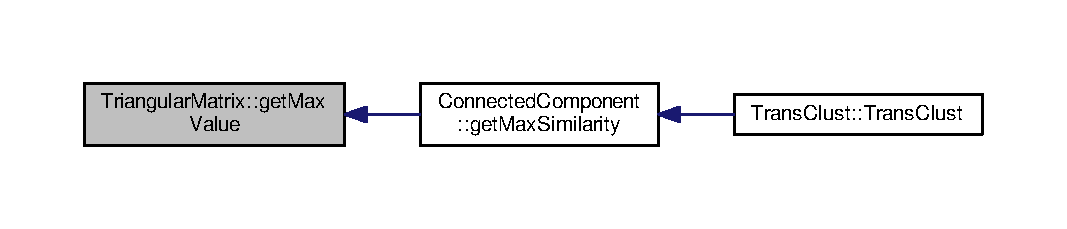
\includegraphics[width=350pt]{classTriangularMatrix_a1f93bf63a6c6c09d5130ab3111aaab05_icgraph}
\end{center}
\end{figure}


\hypertarget{classTriangularMatrix_adfcd136b2d1e437fe86eee93e8d5dcee}{\index{Triangular\-Matrix@{Triangular\-Matrix}!get\-Min\-Value@{get\-Min\-Value}}
\index{get\-Min\-Value@{get\-Min\-Value}!TriangularMatrix@{Triangular\-Matrix}}
\subsubsection[{get\-Min\-Value}]{\setlength{\rightskip}{0pt plus 5cm}float Triangular\-Matrix\-::get\-Min\-Value (
\begin{DoxyParamCaption}
{}
\end{DoxyParamCaption}
) const\hspace{0.3cm}{\ttfamily [inline]}}}\label{classTriangularMatrix_adfcd136b2d1e437fe86eee93e8d5dcee}


Here is the caller graph for this function\-:\nopagebreak
\begin{figure}[H]
\begin{center}
\leavevmode
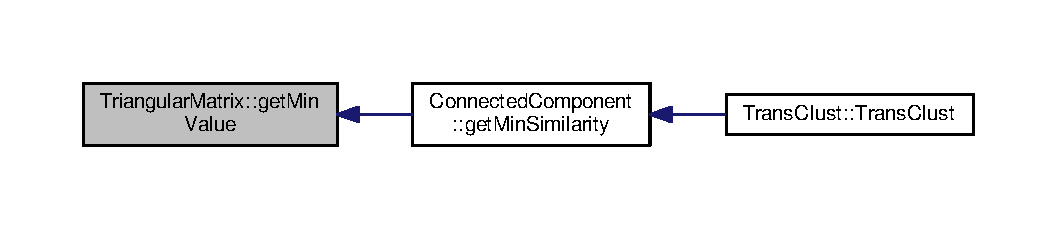
\includegraphics[width=350pt]{classTriangularMatrix_adfcd136b2d1e437fe86eee93e8d5dcee_icgraph}
\end{center}
\end{figure}


\hypertarget{classTriangularMatrix_a5040afab8fb04018c02dc2532401fab1}{\index{Triangular\-Matrix@{Triangular\-Matrix}!get\-Num\-Objects@{get\-Num\-Objects}}
\index{get\-Num\-Objects@{get\-Num\-Objects}!TriangularMatrix@{Triangular\-Matrix}}
\subsubsection[{get\-Num\-Objects}]{\setlength{\rightskip}{0pt plus 5cm}const unsigned Triangular\-Matrix\-::get\-Num\-Objects (
\begin{DoxyParamCaption}
{}
\end{DoxyParamCaption}
) const\hspace{0.3cm}{\ttfamily [inline]}}}\label{classTriangularMatrix_a5040afab8fb04018c02dc2532401fab1}


Here is the caller graph for this function\-:\nopagebreak
\begin{figure}[H]
\begin{center}
\leavevmode
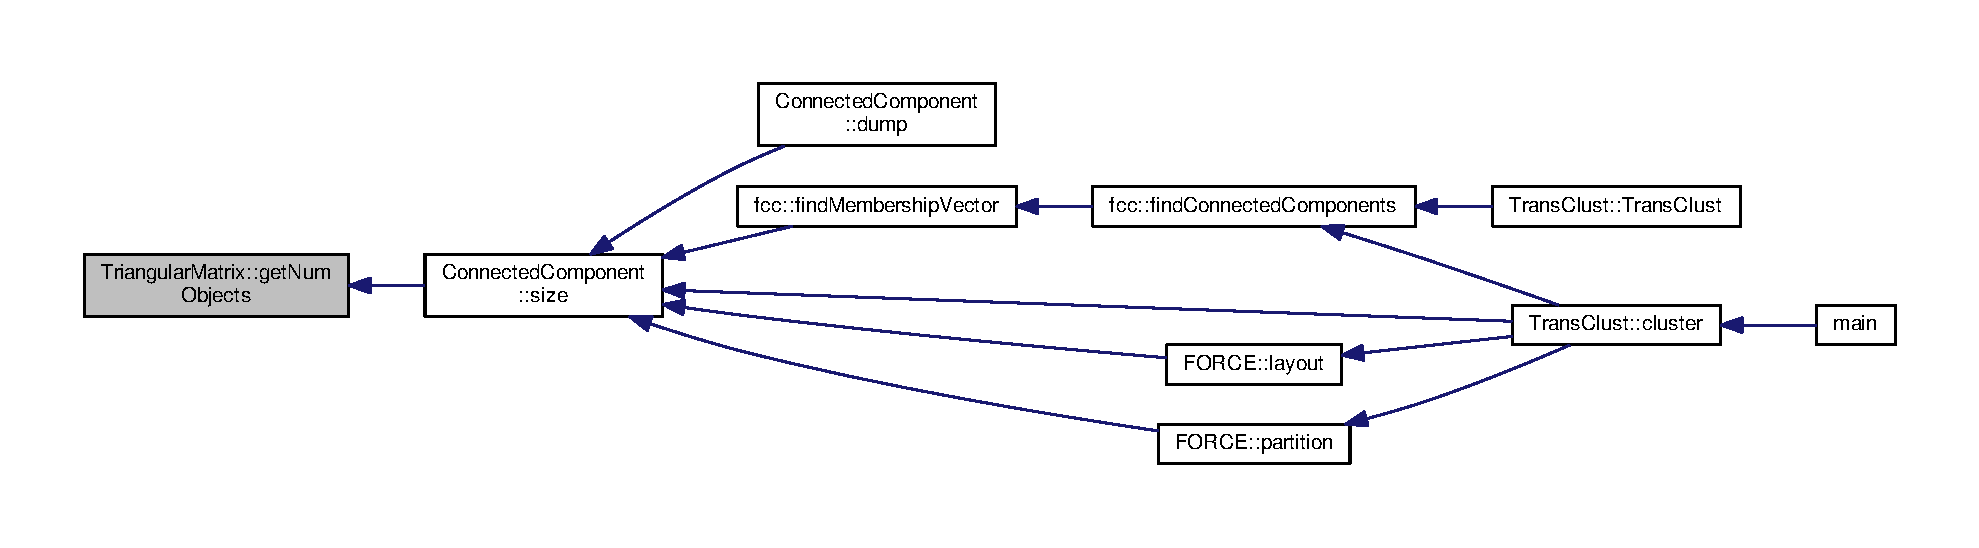
\includegraphics[width=350pt]{classTriangularMatrix_a5040afab8fb04018c02dc2532401fab1_icgraph}
\end{center}
\end{figure}


\hypertarget{classTriangularMatrix_aced0b17dd812119356bc0a0e601b3fff}{\index{Triangular\-Matrix@{Triangular\-Matrix}!get\-Object\-Id@{get\-Object\-Id}}
\index{get\-Object\-Id@{get\-Object\-Id}!TriangularMatrix@{Triangular\-Matrix}}
\subsubsection[{get\-Object\-Id}]{\setlength{\rightskip}{0pt plus 5cm}const unsigned Triangular\-Matrix\-::get\-Object\-Id (
\begin{DoxyParamCaption}
\item[{unsigned}]{i}
\end{DoxyParamCaption}
) const\hspace{0.3cm}{\ttfamily [inline]}}}\label{classTriangularMatrix_aced0b17dd812119356bc0a0e601b3fff}


Here is the caller graph for this function\-:\nopagebreak
\begin{figure}[H]
\begin{center}
\leavevmode
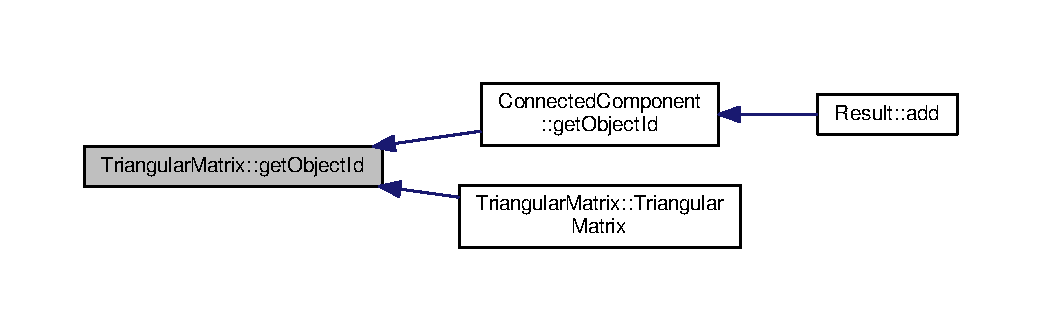
\includegraphics[width=350pt]{classTriangularMatrix_aced0b17dd812119356bc0a0e601b3fff_icgraph}
\end{center}
\end{figure}


\hypertarget{classTriangularMatrix_a13b74e86bd006c503c9a2958b2b93a3a}{\index{Triangular\-Matrix@{Triangular\-Matrix}!get\-Object\-Name@{get\-Object\-Name}}
\index{get\-Object\-Name@{get\-Object\-Name}!TriangularMatrix@{Triangular\-Matrix}}
\subsubsection[{get\-Object\-Name}]{\setlength{\rightskip}{0pt plus 5cm}const std\-::string Triangular\-Matrix\-::get\-Object\-Name (
\begin{DoxyParamCaption}
\item[{unsigned}]{i}
\end{DoxyParamCaption}
) const\hspace{0.3cm}{\ttfamily [inline]}}}\label{classTriangularMatrix_a13b74e86bd006c503c9a2958b2b93a3a}


Here is the caller graph for this function\-:\nopagebreak
\begin{figure}[H]
\begin{center}
\leavevmode
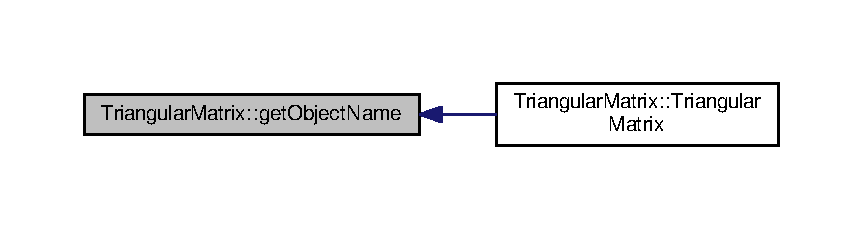
\includegraphics[width=350pt]{classTriangularMatrix_a13b74e86bd006c503c9a2958b2b93a3a_icgraph}
\end{center}
\end{figure}


\hypertarget{classTriangularMatrix_a8786092d7b7c58613b6e19384c7ebfcb}{\index{Triangular\-Matrix@{Triangular\-Matrix}!get\-Object\-Names@{get\-Object\-Names}}
\index{get\-Object\-Names@{get\-Object\-Names}!TriangularMatrix@{Triangular\-Matrix}}
\subsubsection[{get\-Object\-Names}]{\setlength{\rightskip}{0pt plus 5cm}const std\-::vector$<$std\-::string$>$\& Triangular\-Matrix\-::get\-Object\-Names (
\begin{DoxyParamCaption}
{}
\end{DoxyParamCaption}
) const\hspace{0.3cm}{\ttfamily [inline]}}}\label{classTriangularMatrix_a8786092d7b7c58613b6e19384c7ebfcb}


Here is the caller graph for this function\-:\nopagebreak
\begin{figure}[H]
\begin{center}
\leavevmode
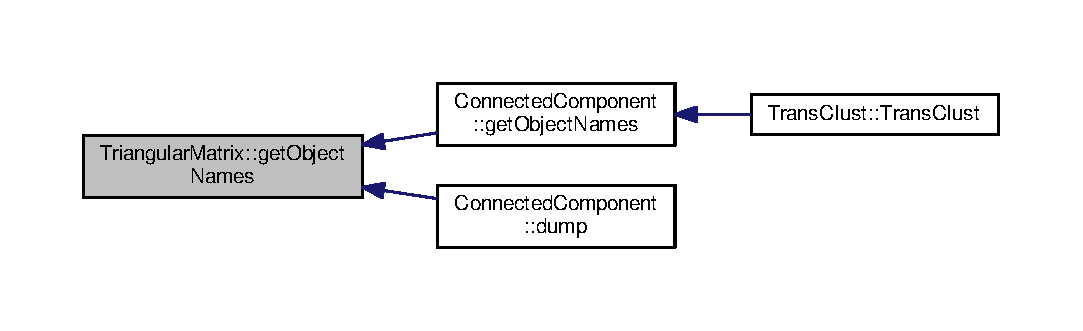
\includegraphics[width=350pt]{classTriangularMatrix_a8786092d7b7c58613b6e19384c7ebfcb_icgraph}
\end{center}
\end{figure}


\hypertarget{classTriangularMatrix_adba103bc50d20c4fd623ee0d00d94cc4}{\index{Triangular\-Matrix@{Triangular\-Matrix}!operator()@{operator()}}
\index{operator()@{operator()}!TriangularMatrix@{Triangular\-Matrix}}
\subsubsection[{operator()}]{\setlength{\rightskip}{0pt plus 5cm}float\& Triangular\-Matrix\-::operator() (
\begin{DoxyParamCaption}
\item[{unsigned}]{i, }
\item[{unsigned}]{j}
\end{DoxyParamCaption}
)\hspace{0.3cm}{\ttfamily [inline]}}}\label{classTriangularMatrix_adba103bc50d20c4fd623ee0d00d94cc4}
\hypertarget{classTriangularMatrix_a61d203934af7655e8406b623326cf8e1}{\index{Triangular\-Matrix@{Triangular\-Matrix}!operator()@{operator()}}
\index{operator()@{operator()}!TriangularMatrix@{Triangular\-Matrix}}
\subsubsection[{operator()}]{\setlength{\rightskip}{0pt plus 5cm}const float\& Triangular\-Matrix\-::operator() (
\begin{DoxyParamCaption}
\item[{unsigned}]{i, }
\item[{unsigned}]{j}
\end{DoxyParamCaption}
) const\hspace{0.3cm}{\ttfamily [inline]}}}\label{classTriangularMatrix_a61d203934af7655e8406b623326cf8e1}


The documentation for this class was generated from the following files\-:\begin{DoxyCompactItemize}
\item 
include/\hyperlink{TriangularMatrix_8hpp}{Triangular\-Matrix.\-hpp}\item 
src/\hyperlink{TriangularMatrix_8cpp}{Triangular\-Matrix.\-cpp}\end{DoxyCompactItemize}

\chapter{File Documentation}
\hypertarget{ClusteringResult_8hpp}{\section{include/\-Clustering\-Result.hpp File Reference}
\label{ClusteringResult_8hpp}\index{include/\-Clustering\-Result.\-hpp@{include/\-Clustering\-Result.\-hpp}}
}
{\ttfamily \#include $<$vector$>$}\\*
{\ttfamily \#include \char`\"{}Connected\-Component.\-hpp\char`\"{}}\\*
Include dependency graph for Clustering\-Result.\-hpp\-:\nopagebreak
\begin{figure}[H]
\begin{center}
\leavevmode
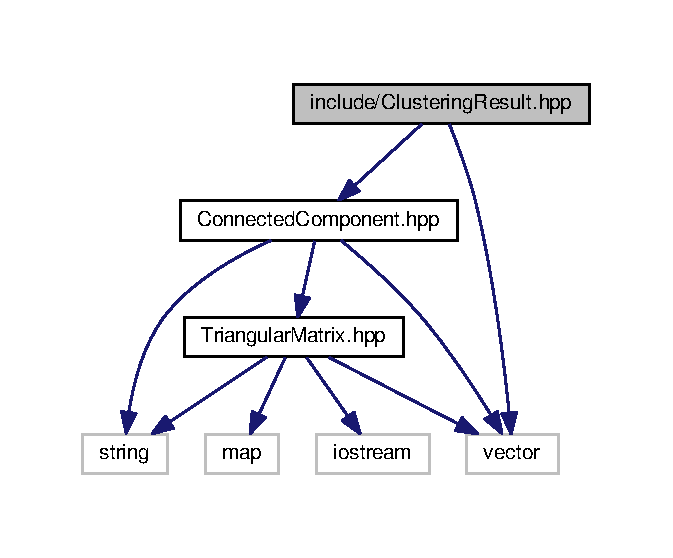
\includegraphics[width=323pt]{ClusteringResult_8hpp__incl}
\end{center}
\end{figure}
This graph shows which files directly or indirectly include this file\-:
\nopagebreak
\begin{figure}[H]
\begin{center}
\leavevmode
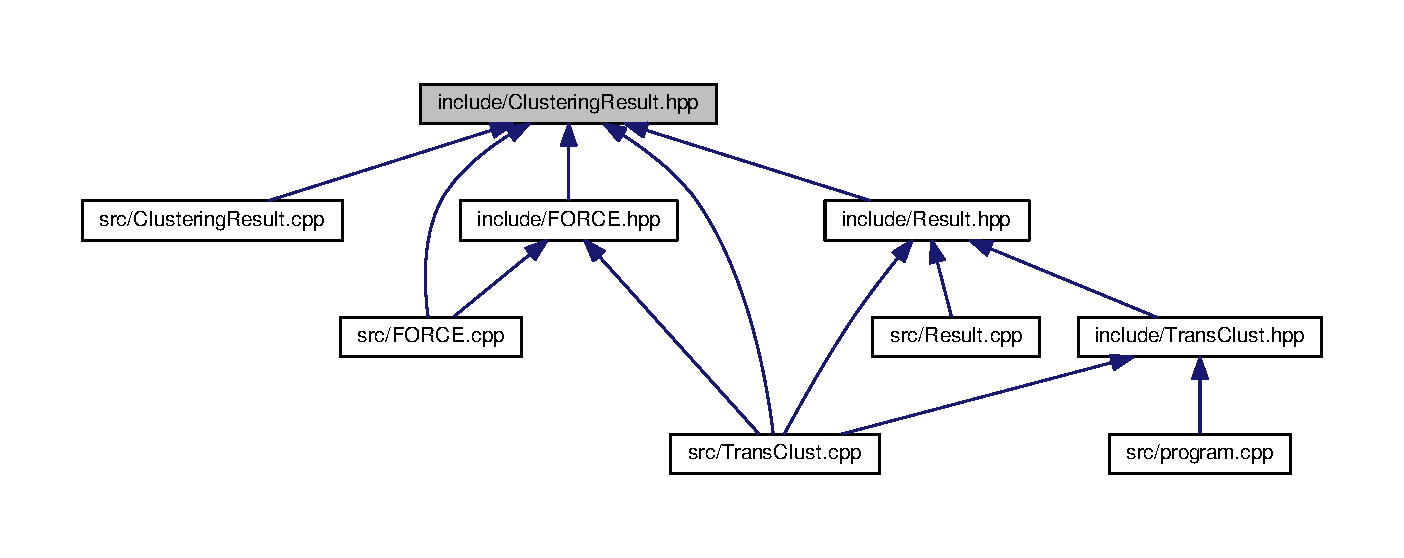
\includegraphics[width=350pt]{ClusteringResult_8hpp__dep__incl}
\end{center}
\end{figure}
\subsection*{Classes}
\begin{DoxyCompactItemize}
\item 
class \hyperlink{classClusteringResult}{Clustering\-Result}
\end{DoxyCompactItemize}

\hypertarget{ConnectedComponent_8hpp}{\section{include/\-Connected\-Component.hpp File Reference}
\label{ConnectedComponent_8hpp}\index{include/\-Connected\-Component.\-hpp@{include/\-Connected\-Component.\-hpp}}
}
{\ttfamily \#include $<$string$>$}\\*
{\ttfamily \#include $<$vector$>$}\\*
{\ttfamily \#include \char`\"{}Triangular\-Matrix.\-hpp\char`\"{}}\\*
Include dependency graph for Connected\-Component.\-hpp\-:\nopagebreak
\begin{figure}[H]
\begin{center}
\leavevmode
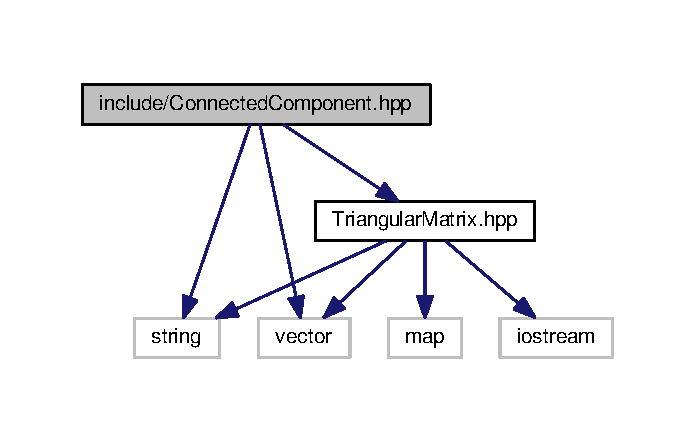
\includegraphics[width=334pt]{ConnectedComponent_8hpp__incl}
\end{center}
\end{figure}
This graph shows which files directly or indirectly include this file\-:
\nopagebreak
\begin{figure}[H]
\begin{center}
\leavevmode
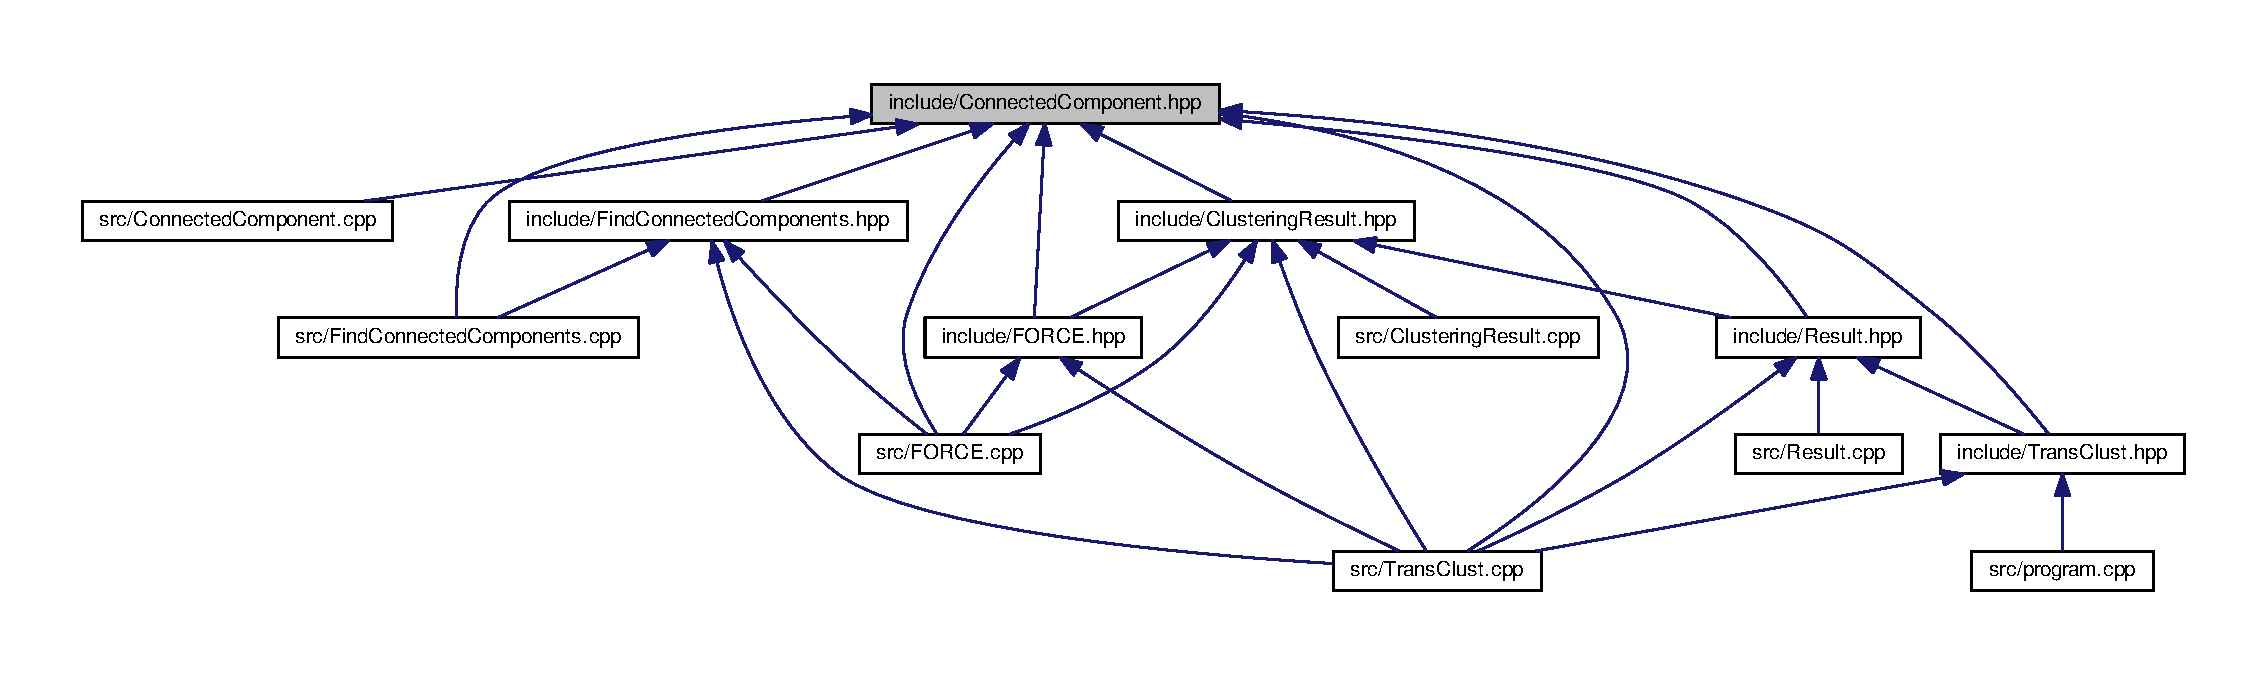
\includegraphics[width=350pt]{ConnectedComponent_8hpp__dep__incl}
\end{center}
\end{figure}
\subsection*{Classes}
\begin{DoxyCompactItemize}
\item 
class \hyperlink{classConnectedComponent}{Connected\-Component}
\end{DoxyCompactItemize}
\subsection*{Functions}
\begin{DoxyCompactItemize}
\item 
static unsigned \hyperlink{ConnectedComponent_8hpp_a6a69b0f8fa6235cb9ec103446b24a274}{\-\_\-cc\-\_\-id} (0)
\end{DoxyCompactItemize}


\subsection{Function Documentation}
\hypertarget{ConnectedComponent_8hpp_a6a69b0f8fa6235cb9ec103446b24a274}{\index{Connected\-Component.\-hpp@{Connected\-Component.\-hpp}!\-\_\-cc\-\_\-id@{\-\_\-cc\-\_\-id}}
\index{\-\_\-cc\-\_\-id@{\-\_\-cc\-\_\-id}!ConnectedComponent.hpp@{Connected\-Component.\-hpp}}
\subsubsection[{\-\_\-cc\-\_\-id}]{\setlength{\rightskip}{0pt plus 5cm}static unsigned \-\_\-cc\-\_\-id (
\begin{DoxyParamCaption}
\item[{0}]{}
\end{DoxyParamCaption}
)\hspace{0.3cm}{\ttfamily [static]}}}\label{ConnectedComponent_8hpp_a6a69b0f8fa6235cb9ec103446b24a274}

\hypertarget{FindConnectedComponents_8hpp}{\section{include/\-Find\-Connected\-Components.hpp File Reference}
\label{FindConnectedComponents_8hpp}\index{include/\-Find\-Connected\-Components.\-hpp@{include/\-Find\-Connected\-Components.\-hpp}}
}
{\ttfamily \#include $<$vector$>$}\\*
{\ttfamily \#include $<$queue$>$}\\*
{\ttfamily \#include \char`\"{}Connected\-Component.\-hpp\char`\"{}}\\*
Include dependency graph for Find\-Connected\-Components.\-hpp\-:\nopagebreak
\begin{figure}[H]
\begin{center}
\leavevmode
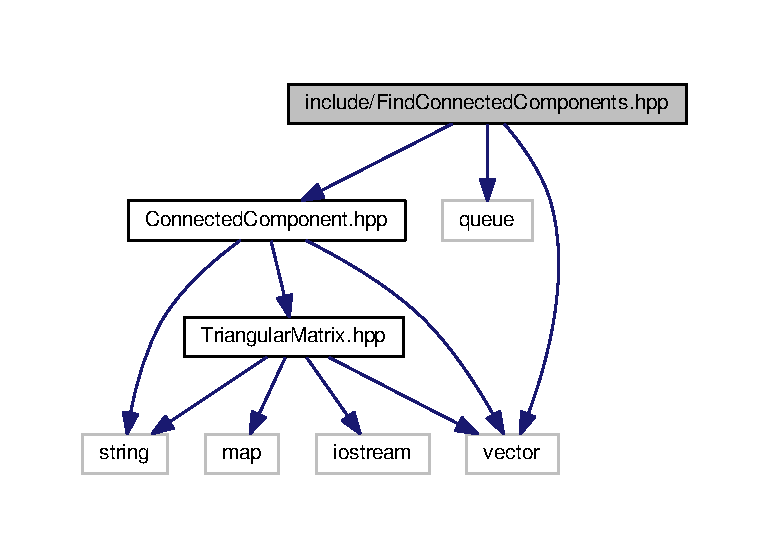
\includegraphics[width=350pt]{FindConnectedComponents_8hpp__incl}
\end{center}
\end{figure}
This graph shows which files directly or indirectly include this file\-:\nopagebreak
\begin{figure}[H]
\begin{center}
\leavevmode
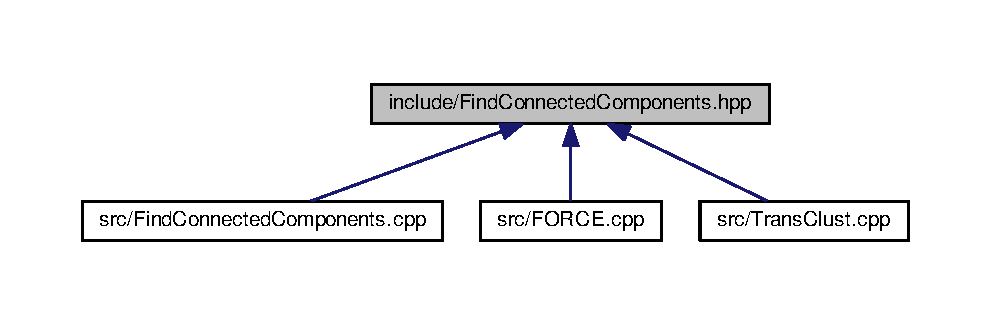
\includegraphics[width=350pt]{FindConnectedComponents_8hpp__dep__incl}
\end{center}
\end{figure}
\subsection*{Namespaces}
\begin{DoxyCompactItemize}
\item 
\hyperlink{namespacefcc}{fcc}
\end{DoxyCompactItemize}
\subsection*{Functions}
\begin{DoxyCompactItemize}
\item 
void \hyperlink{namespacefcc_a7bb6ac8b965c5b8273285865d31af94d}{fcc\-::find\-Connected\-Components} (const \hyperlink{classConnectedComponent}{Connected\-Component} \&cc, std\-::queue$<$ \hyperlink{classConnectedComponent}{Connected\-Component} $>$ \&ccs, const float threshold)
\item 
std\-::vector$<$ std\-::vector\\*
$<$ unsigned $>$ $>$ \hyperlink{namespacefcc_af21d20aac08ecb1a28be9244dbb525fe}{fcc\-::find\-Membership\-Vector} (const \hyperlink{classConnectedComponent}{Connected\-Component} \&cc, const float threshold)
\item 
void \hyperlink{namespacefcc_aabaae257f8d62570bfc4289a9483289e}{fcc\-::find\-Connected\-Components} (const \hyperlink{classConnectedComponent}{Connected\-Component} \&cc, const std\-::vector$<$ std\-::vector$<$ float $>$$>$ \&pos, std\-::vector$<$ \hyperlink{classConnectedComponent}{Connected\-Component} $>$ \&ccs, const float threshold)
\item 
std\-::vector$<$ std\-::vector\\*
$<$ unsigned $>$ $>$ \hyperlink{namespacefcc_a57c1a3d97ea9e78ea37513476c1b2f60}{fcc\-::find\-Membership\-Vector} (const \hyperlink{classConnectedComponent}{Connected\-Component} \&cc, const std\-::vector$<$ std\-::vector$<$ float $>$$>$ \&pos, std\-::vector$<$ \hyperlink{classConnectedComponent}{Connected\-Component} $>$ \&ccs, const float threshold)
\end{DoxyCompactItemize}

\hypertarget{FORCE_8hpp}{\section{include/\-F\-O\-R\-C\-E.hpp File Reference}
\label{FORCE_8hpp}\index{include/\-F\-O\-R\-C\-E.\-hpp@{include/\-F\-O\-R\-C\-E.\-hpp}}
}
{\ttfamily \#include $<$vector$>$}\\*
{\ttfamily \#include $<$math.\-h$>$}\\*
{\ttfamily \#include $<$iostream$>$}\\*
{\ttfamily \#include \char`\"{}Connected\-Component.\-hpp\char`\"{}}\\*
{\ttfamily \#include \char`\"{}Clustering\-Result.\-hpp\char`\"{}}\\*
Include dependency graph for F\-O\-R\-C\-E.\-hpp\-:\nopagebreak
\begin{figure}[H]
\begin{center}
\leavevmode
\includegraphics[width=350pt]{FORCE_8hpp__incl}
\end{center}
\end{figure}
This graph shows which files directly or indirectly include this file\-:\nopagebreak
\begin{figure}[H]
\begin{center}
\leavevmode
\includegraphics[width=285pt]{FORCE_8hpp__dep__incl}
\end{center}
\end{figure}
\subsection*{Namespaces}
\begin{DoxyCompactItemize}
\item 
\hyperlink{namespaceFORCE}{F\-O\-R\-C\-E}
\end{DoxyCompactItemize}
\subsection*{Functions}
\begin{DoxyCompactItemize}
\item 
float \hyperlink{namespaceFORCE_aa98e605135ced38fe09c8c97a2597af0}{F\-O\-R\-C\-E\-::dist} (std\-::vector$<$ std\-::vector$<$ float $>$$>$ \&pos, unsigned i, unsigned j)
\item 
void \hyperlink{namespaceFORCE_a98853866c9b35b686d06faaeaffedff4}{F\-O\-R\-C\-E\-::layout} (const \hyperlink{classConnectedComponent}{Connected\-Component} \&cc, std\-::vector$<$ std\-::vector$<$ float $>$$>$ \&pos, float p, float f\-\_\-att, float f\-\_\-rep, unsigned R, float start\-\_\-t, unsigned dim)
\item 
\hyperlink{classClusteringResult}{Clustering\-Result} \hyperlink{namespaceFORCE_a0c6a6dbc5e4c7cc9d9c33dd884034941}{F\-O\-R\-C\-E\-::partition} (const \hyperlink{classConnectedComponent}{Connected\-Component} \&cc, std\-::vector$<$ std\-::vector$<$ float $>$$>$ \&pos, float d\-\_\-init, float d\-\_\-maximal, float s\-\_\-init, float f\-\_\-s)
\item 
std\-::vector$<$ std\-::vector\\*
$<$ unsigned $>$ $>$ \hyperlink{namespaceFORCE_ac58f3224b8bcfdce18f57ed692278f00}{F\-O\-R\-C\-E\-::geometric\-Linking} (std\-::vector$<$ std\-::vector$<$ float $>$$>$ \&pos, const float max\-Dist, const std\-::vector$<$ std\-::vector$<$ unsigned $>$$>$ \&objects)
\item 
void \hyperlink{namespaceFORCE_a4757f1fe7991d161f1deb3dafa1b933e}{F\-O\-R\-C\-E\-::\-D\-E\-B\-U\-G\-\_\-delta} (const \hyperlink{classConnectedComponent}{Connected\-Component} \&cc, std\-::vector$<$ std\-::vector$<$ float $>$$>$ \&pos, std\-::vector$<$ std\-::vector$<$ float $>$$>$ \&delta, unsigned r)
\item 
void \hyperlink{namespaceFORCE_a2a8c27faac3bf131cbf45212b723286e}{F\-O\-R\-C\-E\-::\-D\-E\-B\-U\-G\-\_\-position} (const \hyperlink{classConnectedComponent}{Connected\-Component} \&cc, std\-::vector$<$ std\-::vector$<$ float $>$$>$ \&pos, float r)
\item 
void \hyperlink{namespaceFORCE_a91fbcba5dd9ef801ef9c1b145722d7e1}{F\-O\-R\-C\-E\-::\-D\-E\-B\-U\-G\-\_\-linking} (std\-::vector$<$ unsigned $>$ membership, std\-::vector$<$ std\-::vector$<$ float $>$$>$ pos, float threshold, unsigned id)
\end{DoxyCompactItemize}

\hypertarget{Result_8hpp}{\section{include/\-Result.hpp File Reference}
\label{Result_8hpp}\index{include/\-Result.\-hpp@{include/\-Result.\-hpp}}
}
{\ttfamily \#include $<$vector$>$}\\*
{\ttfamily \#include $<$set$>$}\\*
{\ttfamily \#include \char`\"{}Connected\-Component.\-hpp\char`\"{}}\\*
{\ttfamily \#include \char`\"{}Clustering\-Result.\-hpp\char`\"{}}\\*
Include dependency graph for Result.\-hpp\-:\nopagebreak
\begin{figure}[H]
\begin{center}
\leavevmode
\includegraphics[width=350pt]{Result_8hpp__incl}
\end{center}
\end{figure}
This graph shows which files directly or indirectly include this file\-:
\nopagebreak
\begin{figure}[H]
\begin{center}
\leavevmode
\includegraphics[width=343pt]{Result_8hpp__dep__incl}
\end{center}
\end{figure}
\subsection*{Classes}
\begin{DoxyCompactItemize}
\item 
class \hyperlink{classResult}{Result}
\end{DoxyCompactItemize}

\hypertarget{TransClust_8hpp}{\section{include/\-Trans\-Clust.hpp File Reference}
\label{TransClust_8hpp}\index{include/\-Trans\-Clust.\-hpp@{include/\-Trans\-Clust.\-hpp}}
}
{\ttfamily \#include $<$string$>$}\\*
{\ttfamily \#include $<$queue$>$}\\*
{\ttfamily \#include $<$vector$>$}\\*
{\ttfamily \#include $<$map$>$}\\*
{\ttfamily \#include $<$Connected\-Component.\-hpp$>$}\\*
{\ttfamily \#include \char`\"{}Result.\-hpp\char`\"{}}\\*
Include dependency graph for Trans\-Clust.\-hpp\-:\nopagebreak
\begin{figure}[H]
\begin{center}
\leavevmode
\includegraphics[width=350pt]{TransClust_8hpp__incl}
\end{center}
\end{figure}
This graph shows which files directly or indirectly include this file\-:\nopagebreak
\begin{figure}[H]
\begin{center}
\leavevmode
\includegraphics[width=285pt]{TransClust_8hpp__dep__incl}
\end{center}
\end{figure}
\subsection*{Classes}
\begin{DoxyCompactItemize}
\item 
class \hyperlink{classTransClust}{Trans\-Clust}
\end{DoxyCompactItemize}

\hypertarget{TriangularMatrix_8hpp}{\section{include/\-Triangular\-Matrix.hpp File Reference}
\label{TriangularMatrix_8hpp}\index{include/\-Triangular\-Matrix.\-hpp@{include/\-Triangular\-Matrix.\-hpp}}
}
{\ttfamily \#include $<$string$>$}\\*
{\ttfamily \#include $<$map$>$}\\*
{\ttfamily \#include $<$vector$>$}\\*
{\ttfamily \#include $<$iostream$>$}\\*
Include dependency graph for Triangular\-Matrix.\-hpp\-:\nopagebreak
\begin{figure}[H]
\begin{center}
\leavevmode
\includegraphics[width=308pt]{TriangularMatrix_8hpp__incl}
\end{center}
\end{figure}
This graph shows which files directly or indirectly include this file\-:
\nopagebreak
\begin{figure}[H]
\begin{center}
\leavevmode
\includegraphics[width=350pt]{TriangularMatrix_8hpp__dep__incl}
\end{center}
\end{figure}
\subsection*{Classes}
\begin{DoxyCompactItemize}
\item 
class \hyperlink{classTriangularMatrix}{Triangular\-Matrix}
\end{DoxyCompactItemize}

\hypertarget{ClusteringResult_8cpp}{\section{src/\-Clustering\-Result.cpp File Reference}
\label{ClusteringResult_8cpp}\index{src/\-Clustering\-Result.\-cpp@{src/\-Clustering\-Result.\-cpp}}
}
{\ttfamily \#include \char`\"{}Clustering\-Result.\-hpp\char`\"{}}\\*
Include dependency graph for Clustering\-Result.\-cpp\-:\nopagebreak
\begin{figure}[H]
\begin{center}
\leavevmode
\includegraphics[width=314pt]{ClusteringResult_8cpp__incl}
\end{center}
\end{figure}

\hypertarget{ConnectedComponent_8cpp}{\section{src/\-Connected\-Component.cpp File Reference}
\label{ConnectedComponent_8cpp}\index{src/\-Connected\-Component.\-cpp@{src/\-Connected\-Component.\-cpp}}
}
{\ttfamily \#include \char`\"{}Connected\-Component.\-hpp\char`\"{}}\\*
Include dependency graph for Connected\-Component.\-cpp\-:\nopagebreak
\begin{figure}[H]
\begin{center}
\leavevmode
\includegraphics[width=325pt]{ConnectedComponent_8cpp__incl}
\end{center}
\end{figure}

\hypertarget{FindConnectedComponents_8cpp}{\section{src/\-Find\-Connected\-Components.cpp File Reference}
\label{FindConnectedComponents_8cpp}\index{src/\-Find\-Connected\-Components.\-cpp@{src/\-Find\-Connected\-Components.\-cpp}}
}
{\ttfamily \#include $<$Find\-Connected\-Components.\-hpp$>$}\\*
{\ttfamily \#include $<$Connected\-Component.\-hpp$>$}\\*
{\ttfamily \#include $<$math.\-h$>$}\\*
{\ttfamily \#include $<$iomanip$>$}\\*
{\ttfamily \#include $<$limits$>$}\\*
Include dependency graph for Find\-Connected\-Components.\-cpp\-:\nopagebreak
\begin{figure}[H]
\begin{center}
\leavevmode
\includegraphics[width=350pt]{FindConnectedComponents_8cpp__incl}
\end{center}
\end{figure}
\subsection*{Namespaces}
\begin{DoxyCompactItemize}
\item 
\hyperlink{namespacefcc}{fcc}
\end{DoxyCompactItemize}
\subsection*{Functions}
\begin{DoxyCompactItemize}
\item 
void \hyperlink{namespacefcc_a7bb6ac8b965c5b8273285865d31af94d}{fcc\-::find\-Connected\-Components} (const \hyperlink{classConnectedComponent}{Connected\-Component} \&cc, std\-::queue$<$ \hyperlink{classConnectedComponent}{Connected\-Component} $>$ \&ccs, const float threshold)
\item 
std\-::vector$<$ std\-::vector\\*
$<$ unsigned $>$ $>$ \hyperlink{namespacefcc_af21d20aac08ecb1a28be9244dbb525fe}{fcc\-::find\-Membership\-Vector} (const \hyperlink{classConnectedComponent}{Connected\-Component} \&cc, const float threshold)
\end{DoxyCompactItemize}

\hypertarget{FORCE_8cpp}{\section{src/\-F\-O\-R\-C\-E.cpp File Reference}
\label{FORCE_8cpp}\index{src/\-F\-O\-R\-C\-E.\-cpp@{src/\-F\-O\-R\-C\-E.\-cpp}}
}
{\ttfamily \#include $<$math.\-h$>$}\\*
{\ttfamily \#include $<$iomanip$>$}\\*
{\ttfamily \#include $<$iostream$>$}\\*
{\ttfamily \#include $<$random$>$}\\*
{\ttfamily \#include $<$limits$>$}\\*
{\ttfamily \#include $<$queue$>$}\\*
{\ttfamily \#include $<$Connected\-Component.\-hpp$>$}\\*
{\ttfamily \#include $<$Find\-Connected\-Components.\-hpp$>$}\\*
{\ttfamily \#include $<$F\-O\-R\-C\-E.\-hpp$>$}\\*
{\ttfamily \#include $<$Clustering\-Result.\-hpp$>$}\\*
Include dependency graph for F\-O\-R\-C\-E.\-cpp\-:\nopagebreak
\begin{figure}[H]
\begin{center}
\leavevmode
\includegraphics[width=350pt]{FORCE_8cpp__incl}
\end{center}
\end{figure}
\subsection*{Namespaces}
\begin{DoxyCompactItemize}
\item 
\hyperlink{namespaceFORCE}{F\-O\-R\-C\-E}
\end{DoxyCompactItemize}
\subsection*{Functions}
\begin{DoxyCompactItemize}
\item 
float \hyperlink{namespaceFORCE_aa98e605135ced38fe09c8c97a2597af0}{F\-O\-R\-C\-E\-::dist} (std\-::vector$<$ std\-::vector$<$ float $>$$>$ \&pos, unsigned i, unsigned j)
\item 
void \hyperlink{namespaceFORCE_a98853866c9b35b686d06faaeaffedff4}{F\-O\-R\-C\-E\-::layout} (const \hyperlink{classConnectedComponent}{Connected\-Component} \&cc, std\-::vector$<$ std\-::vector$<$ float $>$$>$ \&pos, float p, float f\-\_\-att, float f\-\_\-rep, unsigned R, float start\-\_\-t, unsigned dim)
\item 
\hyperlink{classClusteringResult}{Clustering\-Result} \hyperlink{namespaceFORCE_a0c6a6dbc5e4c7cc9d9c33dd884034941}{F\-O\-R\-C\-E\-::partition} (const \hyperlink{classConnectedComponent}{Connected\-Component} \&cc, std\-::vector$<$ std\-::vector$<$ float $>$$>$ \&pos, float d\-\_\-init, float d\-\_\-maximal, float s\-\_\-init, float f\-\_\-s)
\item 
std\-::vector$<$ std\-::vector\\*
$<$ unsigned $>$ $>$ \hyperlink{namespaceFORCE_ac58f3224b8bcfdce18f57ed692278f00}{F\-O\-R\-C\-E\-::geometric\-Linking} (std\-::vector$<$ std\-::vector$<$ float $>$$>$ \&pos, const float max\-Dist, const std\-::vector$<$ std\-::vector$<$ unsigned $>$$>$ \&objects)
\end{DoxyCompactItemize}

\hypertarget{program_8cpp}{\section{src/program.cpp File Reference}
\label{program_8cpp}\index{src/program.\-cpp@{src/program.\-cpp}}
}
{\ttfamily \#include $<$Trans\-Clust.\-hpp$>$}\\*
{\ttfamily \#include $<$iostream$>$}\\*
{\ttfamily \#include $<$tclap/\-Cmd\-Line.\-h$>$}\\*
Include dependency graph for program.\-cpp\-:\nopagebreak
\begin{figure}[H]
\begin{center}
\leavevmode
\includegraphics[width=350pt]{program_8cpp__incl}
\end{center}
\end{figure}
\subsection*{Functions}
\begin{DoxyCompactItemize}
\item 
int \hyperlink{program_8cpp_a3c04138a5bfe5d72780bb7e82a18e627}{main} (int argc, char $\ast$$\ast$argv)
\end{DoxyCompactItemize}


\subsection{Function Documentation}
\hypertarget{program_8cpp_a3c04138a5bfe5d72780bb7e82a18e627}{\index{program.\-cpp@{program.\-cpp}!main@{main}}
\index{main@{main}!program.cpp@{program.\-cpp}}
\subsubsection[{main}]{\setlength{\rightskip}{0pt plus 5cm}int main (
\begin{DoxyParamCaption}
\item[{int}]{argc, }
\item[{char $\ast$$\ast$}]{argv}
\end{DoxyParamCaption}
)}}\label{program_8cpp_a3c04138a5bfe5d72780bb7e82a18e627}


Here is the call graph for this function\-:\nopagebreak
\begin{figure}[H]
\begin{center}
\leavevmode
\includegraphics[width=350pt]{program_8cpp_a3c04138a5bfe5d72780bb7e82a18e627_cgraph}
\end{center}
\end{figure}



\hypertarget{Result_8cpp}{\section{src/\-Result.cpp File Reference}
\label{Result_8cpp}\index{src/\-Result.\-cpp@{src/\-Result.\-cpp}}
}
{\ttfamily \#include \char`\"{}Result.\-hpp\char`\"{}}\\*
{\ttfamily \#include $<$limits$>$}\\*
{\ttfamily \#include $<$algorithm$>$}\\*
{\ttfamily \#include $<$map$>$}\\*
{\ttfamily \#include $<$iomanip$>$}\\*
Include dependency graph for Result.\-cpp\-:\nopagebreak
\begin{figure}[H]
\begin{center}
\leavevmode
\includegraphics[width=350pt]{Result_8cpp__incl}
\end{center}
\end{figure}

\hypertarget{TransClust_8cpp}{\section{src/\-Trans\-Clust.cpp File Reference}
\label{TransClust_8cpp}\index{src/\-Trans\-Clust.\-cpp@{src/\-Trans\-Clust.\-cpp}}
}
{\ttfamily \#include $<$Trans\-Clust.\-hpp$>$}\\*
{\ttfamily \#include $<$Connected\-Component.\-hpp$>$}\\*
{\ttfamily \#include $<$Find\-Connected\-Components.\-hpp$>$}\\*
{\ttfamily \#include $<$F\-O\-R\-C\-E.\-hpp$>$}\\*
{\ttfamily \#include \char`\"{}Clustering\-Result.\-hpp\char`\"{}}\\*
{\ttfamily \#include \char`\"{}Result.\-hpp\char`\"{}}\\*
Include dependency graph for Trans\-Clust.\-cpp\-:\nopagebreak
\begin{figure}[H]
\begin{center}
\leavevmode
\includegraphics[width=350pt]{TransClust_8cpp__incl}
\end{center}
\end{figure}

\hypertarget{TriangularMatrix_8cpp}{\section{src/\-Triangular\-Matrix.cpp File Reference}
\label{TriangularMatrix_8cpp}\index{src/\-Triangular\-Matrix.\-cpp@{src/\-Triangular\-Matrix.\-cpp}}
}
{\ttfamily \#include $<$Triangular\-Matrix.\-hpp$>$}\\*
{\ttfamily \#include $<$fstream$>$}\\*
{\ttfamily \#include $<$iostream$>$}\\*
{\ttfamily \#include $<$sstream$>$}\\*
{\ttfamily \#include $<$iterator$>$}\\*
{\ttfamily \#include $<$limits$>$}\\*
{\ttfamily \#include $<$utility$>$}\\*
Include dependency graph for Triangular\-Matrix.\-cpp\-:\nopagebreak
\begin{figure}[H]
\begin{center}
\leavevmode
\includegraphics[width=350pt]{TriangularMatrix_8cpp__incl}
\end{center}
\end{figure}

%--- End generated contents ---

% Index
\newpage
\phantomsection
\addcontentsline{toc}{chapter}{Index}
\printindex

\end{document}
